%%%%%%%%%%%%%%%%%%%%%%% file template.tex %%%%%%%%%%%%%%%%%%%%%%%%%
%
% This is a general template file for the LaTeX package SVJour3
% for Springer journals.          Springer Heidelberg 2010/09/16
%
% Copy it to a new file with a new name and use it as the basis
% for your article. Delete % signs as needed.
%
% This template includes a few options for different layouts and
% content for various journals. Please consult a previous issue of
% your journal as needed.
%
%%%%%%%%%%%%%%%%%%%%%%%%%%%%%%%%%%%%%%%%%%%%%%%%%%%%%%%%%%%%%%%%%%%
%
% First comes an example EPS file -- just ignore it and
% proceed on the \documentclass line
% your LaTeX will extract the file if required
%\begin{filecontents*}{example.eps}
%%!PS-Adobe-3.0 EPSF-3.0
%%%BoundingBox: 19 19 221 221
%%%CreationDate: Mon Sep 29 1997
%%%Creator: programmed by hand (JK)
%%%EndComments
%gsave
%newpath
%  20 20 moveto
%  20 220 lineto
%  220 220 lineto
%  220 20 lineto
%closepath
%2 setlinewidth
%gsave
%  .4 setgray fill
%grestore
%stroke
%grestore
%\end{filecontents*}
%
\RequirePackage{fix-cm}
%
\documentclass{svjour3}                     % onecolumn (standard format)
%\documentclass[smallcondensed]{svjour3}     % onecolumn (ditto)
%\documentclass[smallextended]{svjour3}       % onecolumn (second format)
%\documentclass[twocolumn]{svjour3}          % twocolumn
%
\smartqed  % flush right qed marks, e.g. at end of proof
%




\usepackage{amssymb}
\setcounter{tocdepth}{3}
\usepackage{graphicx}
\usepackage{algorithm}
\usepackage{algpseudocode}
\usepackage{amsmath}
\usepackage{array}
\usepackage{balance}
\usepackage[hang]{caption}
\usepackage{cite}
\usepackage{color}
\usepackage{graphicx}
\usepackage{indentfirst}
\usepackage{multirow}
\usepackage{rotating}
\usepackage{sistyle}
\usepackage[scriptsize]{subfigure}
\usepackage{tabularx}
\usepackage{url}
\usepackage{verbatim}
\newcommand{\redtext}[1]{\textcolor{red}{#1}}
\floatname{algorithm}{Procedure}
\numberwithin{equation}{section}


%
% \usepackage{mathptmx}      % use Times fonts if available on your TeX system
%
% insert here the call for the packages your document requires
%\usepackage{latexsym}
% etc.
%
% please place your own definitions here and don't use \def but
% \newcommand{}{}
%
% Insert the name of "your journal" with
% \journalname{myjournal}
%

%\setlength{\textwidth}{13cm}


\begin{document}

\title{
Recommending Missing Sensor Values
%Insert your title here%\thanks{Grants or other notes
%about the article that should go on the front page should be
%placed here. General acknowledgments should be placed at the end of the article.}
}

%\titlerunning{Short form of title}        % if too long for running head

\author{ % ntu/intel combined style
Chung-Yi Li  \\ Wei-Lun Su \\ Todd G.\ McKenzie \\ Fu-Chun Hsu \and\\ %students
Shou-De Lin \\ Phillip B.\ Gibbons \\ Jane Yung-jen Hsu %professors + phil
}


\authorrunning{Chung-Yi Li et al.\ }

%\authorrunning{Short form of author list} % if too long for running head

\institute{
Chung-Yi Li, Wei-Lun Su, Todd G.\ McKenzie, Fu-Chun Hsu, Shou-De Lin, Jane Yung-jen Hsu
\at
Department of Computer Science and Information Engineering,\\
National Taiwan University, Taiwan\\
\email{\{r00922051,r00922050,d97041,r94082,sdlin,yjhsu\}@csie.ntu.edu.tw}
\and
Phillip B.\ Gibbons
\at
Intel Labs Pittsburgh, USA\\
\email{phillip.b.gibbons@intel.com}
}

\date{Received: date / Accepted: date}
% The correct dates will be entered by the editor


\maketitle


\begin{abstract}
Data sets gathered from sensor networks often suffer from a significant fraction of missing data, due to issues such as 
communication interference, sensor interference, power depletion, and hardware failure. 
Many standard data analysis tools such as classification engines, time-sequence pattern analysis modules, and even statistical tools are ill-equipped to deal will missing values---hence, there is a need to impute missing readings prior to analysis.

In this paper, we present novel imputation methods that take a ``Recommendation Systems'' view of the problem: 
the sensors and their readings at each time step are viewed as products and user product ratings, 
with the goal of estimating the missing ratings.
Sensor readings differ from product ratings, however, in that the former exhibit high correlation in both time and space.
To incorporate this property, we modify the widely successful Matrix Factorization (MF) approach for recommendation systems 
to model temporal correlations and learn latent relationships among sensors.
We evaluate the approach using two environmental sensor network datasets, one indoor and one outdoor, and
two imputation tasks, corresponding to intermittent readings and failed sensors.
The results show that our Temporally-regularized MF (TR-MF) approach provides significantly higher estimation accuracy than 
both (i) state-of-the-art recommendation models and (ii) state-of-the-art sensor data imputation approaches 
such as the hybrid-KNN model.
Interestingly, adding spatial coordinate information into TR-MF is shown to be ineffective---TR-MF already
captures the latent relationships among sensors, including spatial correlations.

Next, we consider sensor networks with multiple sensor types at each
node.  We present two techniques for extending TR-MF to account for
possible correlations among sensor types (e.g., temperature and
humidity): Multivariate TR-MF and Temporally-regularized Tensor
Factorization.  Our results show that both techniques are
significantly more accurate than prior approaches, and each has its
strengths, depending on the observed variance in the readings.
Finally, we consider a popular data analysis task---building
regression-based prediction models---and show that, compared to prior
approaches, applying our more-accurate imputation techniques leads to
higher-quality prediction models.  

\end{abstract}

%\category{H.4}{Information Systems Applications}{Miscellaneous}
%A category including the fourth, optional field follows...
%\category{D.2.8}{Software Engineering}{Metrics}[complexity measures, performance measures]

%\terms{Delphi theory}

\keywords{missing data recovery, matrix factorization, tensor factorization, temporal regularization, multivariate learning, data imputation}

\section{Introduction}

%\subsection{Problem Statement \redtext{(what is the problem to be solved?)}}
%We develop a centralized method for estimating missing data in sensor network datasets, a procedure which is crucial for subsequent analysis.
%Missing data imputation (a term from Statistics) has a long history, and while there are many existing algorithms which estimate missing sensor data (as documented in Section \ref{sec:rw}), few of these take advantage of the time and inter-sensor correlations inherent in the WSN datasets.
%Furthermore, distributed approaches~\cite{xiao2006space,nowak2003distributed} are often limited to providing estimations or decisions based on sensors in the immediate neighborhood and rely on the deployed sensors having adequate computational power to perform such calculations.
%Not suffering from these issues, the centralized approach we have taken enables a global solution (utilizing all observations available from the sensor network) and provides a vital backdrop for our novel highly-accurate sensor network data imputation technique.

%\subsection{Relevance (why is WSN dataset analysis an important topic?)}
%The increasing pervasiveness of Wireless Sensor Network (WSN) deployments is reflected by the recent coinage of terms such as ``Internet of Things'' and ``Machine-to-Machine'' to describe this growing revolution~\cite{ashton2009internet,gershenfeld2004internet,nokia2004machine,lawton2004machine}.
%Facilitated by a sharp reduction in hardware costs~\cite{estrin2000special}, this growing trend (beyond providing for the admission of new phrases into the vernacular) has led to an explosion in the amount and variety of sensor network todata in need of study.
%For this reason, analysis of WSN data has garnered much attention in recent years~\cite{balazinska2007data}.

%\subsection{Motivation \redtext{(why is data imputation needed for WSN datasets?)}}

% Data sets gathered from sensor networks often suffer from a significant fraction of missing data, due to issues such as 
% communication interference, sensor interference, power depletion, and hardware failure. 
% Many standard data analysis tools such as classification engines, time-sequence pattern analysis modules, and even statistical tools are ill-equipped to deal will missing values---hence, there is a need to impute missing readings prior to analysis.

Wireless sensor networks (WSNs) are especially susceptible to interference,
battery depletion, hardware failures, and other environmental and communications ailments
that lead to data loss.  Datasets gathered from sensor networks are
often missing a significant fraction of the possible readings
(e.g., the Intel Berkeley Research lab dataset~\cite{berkeley2004lab}
is missing roughly 50\% of its readings).
These missing values are problematic for data analysis tools such as
classification engines, time-sequence pattern analysis modules, and
other machine learning tasks, which are often ill-equipped to deal
with missing values.  Support Vector Machine
(SVM)~\cite{vapnik2000nature} and Multiple Regression (MR) analysis,
to name but a few examples, require complete datasets with no missing
values.  Popular statistical packages such as SAS, Stata, and R
provide a few default options for handling missing data, as a
preprocessing step, because the core algorithms require that all data be filled
in.  Typical options are (i) remove the entire ``column'' if there is a
missing value or (ii) fill in the missing value (called {\em
imputation}) using either simple defaults like the average of
neighboring values or utilizing user-written code.  The first option discards
otherwise useful data, and in fact, may discard most of the columns in
datasets with high data loss.  Thus, imputation is a vital tool in the
preparation of sensor data for subsequent analysis. Because the
accuracy of the target data analysis depends on the accuracy of the
imputation, improvements in sensor data imputation can better serve
sensor network deployment objectives.

%We consider the common setting where the goal is to collect all the sensor readings
%in order to perform centralized analysis, while maximizing the lifetime of the WSN.
%Sensor nodes are battery powered and may be energy-harvesting, and will often make
%only a ``best effort'' attempt to transmit their readings back to the centralized 
%collection point.  This contributes to the prevalence of missing data, furthering
%the value of effective imputation techniques.

%\subsection{Background \redtext{(what solutions currently exist?)}}

\subsection{Existing Imputation Techniques}

Imputation techniques applied to sensor data can be divided into three categories by the information utilized:
temporal methods (i.e., estimation using the observations from the target sensor at nearby time steps), 
spatial methods (i.e., estimation using neighboring sensor node observations), 
and spatio-temporal methods. They can be further categorized as hot-deck imputation and prediction models~\cite{Garcia:KNNreview},
as shown in Table~\ref{tbl:methods}.
%Hot-deck imputation methods directly fill in the missing values using either neighbor values or historical records from itself 
%such as the \textit{last-seen} method, while the prediction models exploit a function (involving metrics other than just sensor 
%values) to estimate the missing values. 

%The feasibility of estimating missing sensor observations based on historical data is grounded by the known temporal correlation in WSN data~\cite{akyildiz2004exploiting}.
%Moreover, where there is a potential for global communication issues to affect the availability for sensor node observations \emph{en masse} during a given duration of time, utilizing spatial correlations as a basis for estimation may be not be possible.

\paragraph{Temporal Methods}
{\em Temporal methods} leverage the temporal correlation among
readings by the same sensor node; salient methods include observed
data mean~\cite{madden2005tinydb}, last
seen~\cite{Granger:lastseen}, and linear interpolation. %:
%the estimated value $\hat{y_{it}}$ for sensor $i$ at time $t$ is
%$\hat{y_{it}} = y_{iu} + \frac{y_{iv}-y_{iu}}{T_v-T_u}(t-T_u)$,
%where $y_{iu}$ ($y_{iv}$) at time $T_u$ ($T_v$) is the first 
%observation for sensor $i$ prior to (after, respectively) time $t$.

These methods
suffer, however, when there are long temporal gaps in observations for a given
sensor; such gaps can be frequent in WSNs due to power depletion in
energy-harvesting sensors, long-lived communication ailments, etc.  
As a result, the usefulness of temporal imputation
methods drops rapidly as the number of consecutively missing readings
becomes large.

% (i.e., as can happen when intermittent communications starvation occurs in large WSNs).  

\begin{table}
\caption{Salient Methods for Sensor Data Imputation}
\label{tbl:methods}
\centering
{\small
\begin{tabular}{|l|l|l|} \hline
   &{\bf Hot-Deck Imputation}&{\bf Prediction Models}\\ \hline
{\bf Temporal} & Last-seen~\cite{Granger:lastseen}, Mean& Linear Interpolation\\ \hline
\multirow{2}{*}{\bf Spatial}& WARM~\cite{le2005estimating},& DEPM~\cite{li2008data}, K-NN~\cite{pan2010k},\\ 
&FARM~\cite{Gruenwald:FARM}&Multi-Im~\cite{yuan2000multiple}\\\hline
{\bf Spatio-}&STI~\cite{Jian-Zhong:STI}&DESM~\cite{li2008data}, AKE~\cite{pan2010k},\\
{\bf Temporal}&&ImM~\cite{Lim:robust}, EOF~\cite{beckers2003eof} \\\hline \end{tabular}
}
\vspace{-0.1in}
\end{table}

\paragraph{Spatial Methods}
{\em Spatial methods} leverage the spatial correlation among readings
by nearby sensor nodes; salient methods include associations rule
mining (e.g., WARM~\cite{le2005estimating} and
FARM~\cite{Gruenwald:FARM}) 
%\cite{jiang2007estimating} 
and weighted functions of nearby sensors (e.g., DEPM~\cite{li2008data},
K-NN\cite{pan2010k}, and Multi-Im\cite{yuan2000multiple}).

The Data Estimation using Physical Model (DEPM)~\cite{li2008data} method employs the basic laws of Physics to 
design prediction function %as,  
%%\begin{equation}
%$I_K =\sum_{j=1}^M\frac{P_j}{4\pi d^2(I_j,s_k)}$
%%\label{DEPM}
%%\end{equation} 
%where $I_k$ is the intensity of the target sensor value, $j$ represents the neighbor sensors, and P stands for the power radiated from one source to another. 
However, such models are only applicable to limited types of signals, and generally require the precise three-dimensional distance among sensors.

Researchers also propose predicting missing values based on data mining techniques. Window Association Rule Mining (WARM)~\cite{le2005estimating} and Freshness Association Rule Mining (FARM)~\cite{Gruenwald:FARM} study the estimation of missing data based on the association rules among spatially-correlated neighbors. 
Such methods enjoy the advantage of being able to handle categorical sensor data, but the performance is limited in continuous sensor data due to the inherent limitations of association rules.
%(basically, the continuous data needs to be quantized into suitable
%categories for association matches).
%Moreover, the support, confidence of the mined rules need to be predefined by the users which can cause difficulties for building a satisfying model by users without profound knowledge about the environment of deployment. 
%\subsubsection{K-Nearest Neighbours Imputation} 
%  The two major drawbacks of KNN-based model that predicts only from the spatial correlation are: first of all,  they cannot capture temporal correlation, and the second reason is that most of these methods rely on the knowledge of distance between each sensor, which might not be available or accurate in the real world.

The Multi-Im (MI) method~\cite{yuan2000multiple} imputes the missing data by replacing each missing value with a set of plausible values.
%instead of filling in a single value. 
Various methods including multiple linear regression, propensity score method, and Markov chain Monte Carlo method have been used in MI.% The missing data are filled in $M$ times ($M=3-10$~\cite{Little:hotdeck}) 
%to generate $M$ complete datasets, and the results from $M$ generated datasets are averaged to obtain a single prediction~\cite{yuan2000multiple}. 
This model suffers from high computation cost because multiple models have to be learned. Moreover, a poor model might unduly 
contribute to an inferior averaged result. 
%However, this method is criticized on various grounds by WSNs imputation researchers~\cite{jiang2007estimating,Gruenwald:FARM}. 
%First, in sensor data we do not know how many rounds of information to use in order to get the associated information.
%In addition, it is difficult to draw a pool of similar complete cases for a certain round of a certain sensor. 
%Last, it consumes unnecessary time since the sensor data may or may not related to all of the available information.

Generally speaking, there are two ways to obtain the spatial correlation:
from the data or from the spatial coordinates.
We believe the former is a better approach. 
Not only the latter requires reasonably accurate spatial coordinates.
More importantly, it suffers when ailments arise that affect entire
spatial regions (such as large, temporary obstacles to sensing and/or communication).
It also fails to account for barriers or other
sources of sharp environmental gradients.
For example, two nearby sensors, one near a stove and one beside a window, can produce very different values if the stove is in use and the outside temperature is low.
In the end, using spatial coordinates can often lead to worse imputation results
as non-existent or time-varying correlations are imposed between nearby sensors.


%For example, in Figure~\ref{house_floorplan}, we find
%sensors $1$ \& $2$ deployed in the kitchen, next to the stove and
%outside window, respectively. While these sensors are nearby, 
%there may be a large temperature difference between the two if
%the stove is in use and the outside temperature is cold.
%Similarly, sensors $2$ \& $5$
%may be quite uncorrelated despite their relative proximity due to the
%wall between them and the presence of kitchen or laundry appliance
%use.  On the other hand, relatively distant sensors $3$ \& $4$
%may be quite correlated as they are within the same room and both
%near an outside wall. The calculation of
%inter-node signal strength or line of sight distance between nodes
%helps to mitigate these issues, though it is not
%a complete remedy.  In the end, using spatial
%coordinates can often lead to worse imputation results.
% as non-existent or time-varying correlations are imposed between nearby sensors.

%Certain methods consider not strictly the distance between sensors,
%but instead establish a ``neighborhood of influence'' whose size
%becomes a tuning parameter, which adds to the complexity of such methods.

%\begin{figure}[t]
%\centering
%\includegraphics[scale=0.3]{house_floorplan.png}
%\caption{Example home floor plan showing five deployed temperature sensors} \label{house_floorplan}
%\label{fig:example_home_floorplan}
%\vspace{-0.1in}
%\end{figure}

\paragraph{Spatio-Temporal methods}
{\em Spatio-temporal methods} consider both the
temporal and spatial correlation; salient methods include
STI~\cite{Jian-Zhong:STI}, DESM~\cite{li2008data}, 
AKE~\cite{pan2010k}, and Imputation Method~\cite{Lim:robust}.
%These
%have the potential advantage of using both types of correlation in
%imputation, but can suffer from the spatial correlation issues
%discussed above.

The Spatial and Temporal Imputation (STI) algorithm is proposed in~\cite{li2008spatial}. 
For each missing record, STI first checks if some nodes are within the sensing neighborhood, and utilizes
the average of the neighbors to impute the missing value. If no sensors are within the neighborhood, the last seen value of the 
missing sensor is used for imputation. The method favors spatial information over temporal information.

%It has the advantage of simple and fast, but suffers when last seen value is far away from the current time stamp, or when most of the nodes in the sensing region has high missing rate.
%Furthermore, the usage of circular region is problematic as most of the landforms might not be uniformly distributed. Finally, determining the range of the radius is tricky, as a larger radius can cause noise while a smaller one cannot highlight the effectiveness of this model(i.e., the results will be similar to linear interpolation).
%The radius of the region is sometimes too large for sensors whose correlations with the target sensor are low in the sensing range.  
Another spatio-temporal algorithm which relies more on spatial than temporal is the Data Estimation using Statistical Model (DESM)~\cite{li2008data} approach.  
Given two sensors data streams, $\{X_{i1},X_{i2},\dots,X_{im}\}$ and \\ $\{X_{j1},X_{j2},\dots,X_{jm}\}$, and assuming
the value of $X_{i(m+1)}$ is missing,
the prediction on sensor $i$ by its nearest sensor $j$ is:
%\begin{center}
$\hat{X}_{i(m+1)} = (1-\alpha)X_{im} + (\alpha)\hat{z}$
%\end{center}
where $\alpha$ is the Pearson correlation coefficient between the sensor $i$ and $j$, and $\hat{z}$ is the estimation of sensor $i$ 
based on the observation from sensor $j$---it measures the influence of the data sensed by node $i$ on the data of 
the nearest node $j$:
%\begin{center}
$\hat{z} = X_{im}(1+\frac{X_{j(m+1)}-X_{j(m)}}{X_{j(m)}})$
%\end{center}
%The above equation assumes that the sensor $X_i$ and $X_j$ have the similar data fluctuation trend. 
%$\alpha$ is expected to have more impact on the prediction if $X_i$ is more correlated with $X_j$. 
%\begin{equation}
%\label{z-hat}
%\end{equation}
%In DESM, because $\alpha$ is usually high around the target sensor. Therefore, the temporal feature multiplied by $1-\alpha$ holds a very small portion of contribution to the prediction process. It often contradicts the nature that the temporal correlation itself is usually higher than any spatial correlation with other sensors. The performance may becomes bad if the nearest sensor is not the most correlated one, i.e., blocked by a wall.
% \subsubsection{Applying K-nearest neighbour Estimation}

K-nearest neighbors algorithm (KNN) is an intuitive yet effective spatial-correlation-based imputation method. 
It directly uses the weighted average of the neighbor signals to impute the missing data, and has been adopted to successfully 
estimate the missing values of DNA micro-arrays~\cite{Troyanskaya:DNAKNN}.  
%While in WSNs, the sensor data of different nodes is more likely to have some functional relations other than just using sensor values.
Pan~\cite{pan2010k} proposes the Applying K-nearest neighbor Estimation (AKE) algorithm to exploit the spatial correlation in the 
missing sensory data problem. 
AKE adopts a linear regression model to describe the spatial correlation of nodes $i$ and $j$,
%\begin{center}
$y_{it} = \alpha + \beta\cdot y_{jt} + \mu_{jt} $,
%\end{center}
where $y_{it}$ is the observation of sensor $i$ at time $t$, $y_{jt}$ is the data of sensor $j$ at the same time, 
and $\mu_{jt}$ is the random error at time t.   
When the data of sensor $i$ at time $t$ is missing, the estimated value of sensor $i$ by sensor $j$ at the same time is:
%\begin{center}
$\hat{y}_{it}^{(j)} =\hat{\alpha} +\hat{\beta}\cdot y_{jt}$
%\label{ake_j}
%\end{center}
The $\hat{\alpha}$ and $\hat{\beta}$ are the estimated values of $\alpha$ and $\beta$, based on the sample data according to the least squares principle.
%They claim that using a linear combination of the estimation from neighbour sensors can lower the random error caused by only using a single sensor. 
Therefore, given the $m$ nearest neighbor sensors who have values at time $t$[$y_{1t}, y_{2t},\dots, y_{mt}$], the missing value is predicted by :   
% \begin{center}
$ \hat{y}_{it} =\sum_{j=1}^m w_j \cdot \hat{y}_{it}^{(j)}$
 %\label{ake_impute}
% \end{center}
% First they build a matrix 
%\[ \left( \begin{array}{cccc}
%
%\end{array}
%\right)
%\]
where $w_j$ is the weight of sensor $j$ used to predict sensor $i$, and is larger for more highly correlated pairs.
%They adopt the r-square statistics to rank their correlations. The value of $w_j$ is the weighted average of the corresponding 
%r-square values for the $m$ sensors. 

The above models suffer from an issue as they make some unverified assumptions about the data. For example, some models consider temporal correlation as more important than spatial correlation,
%such that the reading of nearby sensors are used only when nearby time steps are missing (or vice versa),
while some assume that sensors of the same distance should have a similar correlation regardless of their 
orientation or other factors.  Such assumptions might or might not hold for various types of data, while imposing them a priori
to the model build might lead to inconsistent results.  The models we propose, however, try to rely less on such a priori 
knowledge, and learn the latent correlation directly from the data.  
%The Imputation Method (ImM)~\cite{Lim:robust}, tries to learn
%the appropriate weighting of temporal and spatial features by considering two temporal predictors, the last-seen predictor
%and an autocorrelation-based temporal linear predictor, and one spatial linear predictor.

\paragraph{Singular Value Decomposition (SVD)-based Methods}
Among the spatio-temporal methods, some are Singular Value Decomposition (SVD)-based methods which are conceptually closer to our
solution. 
SVD-based methods have a significant limitation as they can only be applied to a complete matrix.
Therefore, one needs to somehow first fill in the missing values before conducting such decomposition.
The initial assignment of those missing values, unfortunately, can significantly affect the performance~\cite{koren2009matrix}.
Furthermore, SVD is computationally expensive in general.
In contrast, our approach relies on the factorization process on an incomplete matrix.

%SVD is widely used as a dimension reduction technique.
%It decomposes a fully observed matrix~$\mathbf{R}$ into one diagonal matrix~$\mathbf{D}$ and two unitary matrices~$\mathbf{U}$ and~$\mathbf{V}$ such that
%$\mathbf{R} = \mathbf{U}\mathbf{D}\mathbf{V}^T.$
%The largest $K$ singular values and vectors, $\mathbf{U}_K \mathbf{D}_K \mathbf{V}_K^T$, form the best $K$-rank approximation of $\mathbf{R}$ under the Frobenius Norm.

A salient example of SVD-based approaches for imputation is the Empirical Orthogonal Functions
(EOF) model, which has been applied to oceanographic applications to
solve the problem of missing or unreliable satellite
data~\cite{beckers2003eof}.  EOF first fills in the missing values
(e.g., using all zeros or the mean values) and then performs SVD 
to decompose the matrix. The first $K$ spatial-EOF (i.e., the top-$K$
singular values in SVD) is used to reconstruct the matrix and update the estimation of missing values, 
where $K$ is determined through cross validation over the data.

%In the field of Collaborative Filtering, researchers have already pointed out
%several drawbacks in the SVD-based methods. % when applying to impute missing data. 
%First, given large data, it
%is computational demanding as we need to do the decomposition
%in every iteration. Second, it requires to fill in all missing values
%before the decomposition can be performed, and imperfect initial
%imputation can significantly hurt the final imputation results, in
%particular when the missing data rate is
%high~\cite{koren2009matrix}.

%Hybrid methods of temporal and spatial approaches are less common in the literature.
%For example, the average of the temporal approach of linear interpolation and the spatial approach of multivariate regression has been reported[8].
%Strictly speaking, this approach can be thought of as an ensemble approach between the two methods rather than a fully-integrated approach which considers both temporal and spatial aspects of WSN data.

%\subsection{Research Gap Identification (why are current approaches inadequate?)}
%Accurate imputation of missing sensor network observations is crucial to allow for effective subsequent analysis.
%While there are many existing algorithms which estimate missing data (as documented in the following Related Works section), few of these take advantage of the time and space dependencies inherent in the WSN datasets during the data imputation process.
%As a result, the accuracy of such approaches is limited.

%\subsection{Method Overview \redtext{(what is our approach to bridge the research gap?)}}

\subsection{Our Approach: Collaborative Filtering}

In this paper, we employ a novel {\em Collaborative Filtering} (CF) approach
to sensor data imputation inspired by the field of Recommendation
Systems.  In typical CF approaches, the elements of interest are users
and items (e.g., products), and the values are user ratings of those
items (as in the left-hand side of
Figure~\ref{recommend_imputation}).  Typically, most of the ratings
are missing, and the goal is to predict (impute) the missing ratings
in order to ``recommend'' items to users.  By viewing sensors as
items, users as time steps, and readings as ratings (as illustrated in
Figure~\ref{recommend_imputation}), we can apply CF
techniques to perform sensor data imputation. (Alternatively, sensors
can be viewed as users and items as time steps---the mapping is
irrelevant to the CF formulation.)  In particular, we focus on the
widely successful {\em Matrix Factorization} (MF) technique for CF.

\begin{figure}[H]
\centering
\includegraphics[scale=0.35]{recommend_imputation_timerow.png}
\caption{Bridge from Recommendation Systems to Sensor Data Imputation} 
\label{recommend_imputation}
\vspace{-0.1in}
\end{figure}

Sensor readings differ from user ratings, however, in that the former
exhibit high correlation in both time and space (subject to the above
caveats on space).  To incorporate this property, we first modify MF
to model temporal correlations and learn latent relationships among
sensors.  Specifically, we add temporal-proximity terms to
MF---we call this {\em Temporally-Regularized MF} (TR-MF). 
Similarly, we can also add spatial-proximity terms---we 
call this {\em Spatially-Temporally-Regularized} MF (STR-MF).

Second, we consider sensor networks with multiple sensor types at each node.
We are readily able to exploit such heterogeneous sensor information in our
solution, in contrast to most prior imputation methods that use more ad hoc means.
%Our method incorporates these heterogeneous sensor
%signals (for example, estimating the temperature at a given sensor
%node utilizing the humidity and temperature trends from other
%sensors in the network) to provide more accurate imputation than 
%prior approaches.
We present two techniques for extending 
TR-MF to account for possible correlations among sensor types: {\em Multivariate TR-MF} and 
{\em Temporally-Regularized Tensor Factorization} (TR-TF).

We evaluate our approaches using two environmental sensor network
datasets, one indoor and one outdoor.
%Both datasets record temperature, humidity, and light within its deployed
%environment.  Each dataset has a roughly 50\% initial missing rate (strengthening
%the claim that missing data in WSNs is a common issue), to which we
%additionally cover known observations to use for validation and
%testing purposes.
We study two patterns for missing data: (i) covering
{\em random} readings (modeling intermittent reading failures) and (ii)
covering {\em consecutive} readings for some sensor nodes
(modeling long temporal gaps such as with failed sensors).

Our study shows that TR-MF provides significantly higher estimation accuracy than 
both (i) state-of-the-art recommendation models and (ii) state-of-the-art sensor data imputation approaches 
such as AKE (which is the most accurate prior spatio-temporal method).
Furthermore, our study shows that STR-MF, which adds spatial coordinate information into TR-MF, 
is useful {\em only} in the ``consecutive'' pattern---perhaps surprisingly,
STR-MF is significantly {\em less} accurate than TR-MF in the ``random'' pattern.  This is because TR-MF
effectively leverages the latent relationships among sensors, including any spatial correlations, while avoiding the
pitfalls of spatial-proximity biases.

For the heterogeneous setting, our study shows that both
Multivariate TR-MF and TR-TF can significantly improve the accuracy over TR-MF,
and each has its strengths, depending on the observed variance in the
readings.  Finally, we consider a popular data analysis task---building regression-based prediction models---and show that,
compared to prior approaches for imputation, using TR-MF leads to a much higher quality prediction model.

These results validate our novel approach of equating sensor imputation with recommendation systems.  
%CF approaches such as Matrix Factorization and Tensor Factorization are adept at handling scenarios 
%with large numbers of missing values.
Correlations are captured by grouping correlated sensor nodes and correlated time
steps---unlike prior sensor data imputation approaches, our CF
approaches use this {\em latent} information to impute values, and optimize the evaluation metrics directly. 
Moreover, our CF approaches are global, taking into account all
collected observations, and not overly tied to spatial-proximity
correlations.  
%For example, they can capture the correlations between
%distant sensors $3$ \& $4$ in Figure~\ref{house_floorplan}, while
%grouping sensors $1$, $2$ \& $5$ only if the observed readings warrant
%it.  The CF framework also provides a unified approach to incorporate
%any number of additional sensor types for an even more accurate imputation.

%The reason we believe our method outperforms the results of other methods are as follows.
%\begin{itemize}
%\item A CF approach utilizes {\em latent} information between sensors, e.g., inter-sensor correlation
%\item utilizing heterogeneous sensor information (e.g., utilizing humidity information when estimating temperature) provides additional features which enables a more refined estimation model
%\item we provide an efficient optimization method to learn the inherent model parameters effectively
%\item our method provides a global solution, where all sensor observations available in the dataset can potentially aid in the estimation of a given missing observation
%\end{itemize}

% Given these experimental conditions, we show that our temporal and spatial-oriented collaborative filtering approach to data imputation for WSNs performs more accurately than existing methods such as linear regression and hybrid-kNN.
% In Matrix Factorization, we impose the temporal regularization and Temporal-Regularied MF show the best performance compared to all competitor algorithmss.
% On top of that, we add in spatial regularization and multivariate learning, and we discuss under which circumstance these two are applicable and how they can even improve our models.
% We propose the Tensor Factorization model for missing data recovery. The TF model use additional dimension to capture the correlations of features such as temporal, spatial or heterogeneous signal correlations. The conventional Tensor decomposition technology can only apply on dense tensor. The study of Tensor Factorization model in Collaborative Filtering for recommendation recently, but not practical in sensor network. We  have adapted the TF model for missing value estimation. 

\subsection{Contributions}

In summary, the main contributions of this paper are:
\begin{itemize}
\item We propose viewing sensor data imputation as a recommendation systems problem, and apply state-of-the-art collaborative filtering methods of recommendation systems (namely, matrix and tensor factorization) to the sensor network domain.
\item We augment collaborative filtering with temporal regularization and multi-sensor signals, and provide efficient optimization methods to learn the inherent model parameters effectively.
\item We present an empirical study on two sensor datasets, considering two
missing data patterns corresponding to intermittent readings and failed
sensors. The results show that our proposed approaches provide
significantly higher estimation accuracy than state-of-the-art prior
approaches, and moreover, such accuracy improvements can result in the
generation of higher-quality prediction models.
\end{itemize}

% which finds that our method works well without the incorporation spatial information and that our approach can facilitate the generation of better prediction models

%\subsection{Paper Organization}

%\noindent{\bf Roadmap.}
%%The remainder of our paper is organized as follows.  
%Related work is reviewed in Section~\ref{sec:rw}.  In Sections~\ref{sec:mf} and~\ref{sec:tf} 
%we describe our factorization and multivariate factorization
%approaches to sensor data imputation, respectively. Section \ref{sec:exp} presents our experimental study. 
%Sections \ref{sec:disc} and \ref{sec:conc} provide discussions of our findings and conclusions.

\section{Related Work}
 \begin{table*}
\centering
\caption{Methods for Sensory Data Imputation}
\begin{tabular}{|l|l|l|} \hline
Collection&Hot-Deck Imputation&Prediction Models\\ \hline
\multirow{2}{*} {Temporal} & Last-seen\cite{Granger:lastseen} & Linear Interpolation\\ 
& Mean&\\ \hline
\multirow{3}{*}{Spatial}& WARM\cite{le2005estimating}& DEPM\cite{li2008data}\\ 
&FARM\cite{Gruenwald:FARM}&K-NN\cite{pan2010k}\\ 
&advWARM\cite{jiang:assoication}&\\\hline
\multirow{3}{*}{Hybrid Spatio-Temporal}& &DESM\cite{li2008data}\\ 
&STI\cite{Jian-Zhong:STI}&AKE\cite{pan2010k}\\
&&Ensemble STI\cite{Lim:robust} \\\hline \end{tabular}
\end{table*}
Missing data imputation is the process used to fill the missing data items by determine or assign values\cite{Little:hotdeck}. In wireless sensor network, data is often missing as an entire packet due to communication or power exhaustion problem. Moreover, the physical characteristic of WSNs has shown that there are strong spatial and temporal correlation between sensor nodes and its past historical readings\cite{akyildiz2004exploiting}. Besides, sensor mote is consist of different types of sensors, and some sensors, according to their physical phenomenon, have multivariate correlations\cite{lou:multivariate_gap}. In the research above, they build a probabilistic model to estimate the missing values exploiting spatial, temporal, and multivariate correlation conditioned on the observations. 

According to the strategy deployed to fill in the missing values,  sensory data imputation method can be partitioned into hot-deck imputation, and prediction models\cite{Garcia:KNNreview}. 
Hot-deck imputation methods directly replace the value from either neighbourhood values or historical record from itself such as the \textit{last-seen} method. 
The prediction models provide a function to estimate the missing value using the historical data. 
%\begin{equation}
%y_{it} = f( y_{i(t-1)} , y_{j(t-1})
%\end{equation}

Table 1 summarize the sensory data imputation methods. 
The vertical dimension in table 1 shows whether it exploits the temporal, spatial, or hybrid hybrid of both information. 
The horizontal dimension classifies the methods by how the missing value is produced, either direct substitution or through prediction. 

\subsection{Predictions based on Temporal Information }
\subsubsection{Linear Interpolation}
Linear interpolation(LIN) is a common temporal correlation based technique for missing data prediction. 
It is usually regarded as a baseline method, and has been implemented into some data analysis tools. Mathematically, the estimated value $\hat{y_{it}}$ is:
\begin{equation}
\hat{y_{it}} = y_{iu} + \frac{y_{iv}-y{_iu}}{T_v-T_u}(t-T_u)
\end{equation}
where $y_{iu}$and $y{iv}$ are the previous and the next observations for sensor $i$ at time $t$. 
Linear interpolation method does not considers correlation among sensors.
In general, its performance is acceptable when the missing data are scattered. 
However, the quality of imputation goes down significantly if the sampling rates is low or there are consecutive data missing. 
\subsubsection{Last-seen and moving average}
Imputation based on the last-seen, moving average, and other statistics methods apply on the target sensors generally belong to the temporal-based method as well.
These methods share the advantage of comprehensible and easy implementation. 
However,their performance depends on the sensor data missing pattern as well as sampling rates. For higher sampling rates, these methods perform better.   
\subsection{Prediction based on spatial information}

\subsubsection{Data Estimation using Physical Model}
The physical phenomenon of spatial correlation in sensors measurement can be divided into two categories, the point source and the field source\cite{viran:spatialtemporal}. For point source sensors, the relation between the sensors in a region satisfies physical laws in some event detecting sensors such as light ambient sensors and fire detector. 
Their prediction values are the result of linear superposition by neighbourhood sensors. 
In field source sensor applications, the physical phenomenon is dispersed over the field, for example, the temperature and seismic observation. 
Data Estimation using Physical Model(DEPM)\cite{li2008data} employs the basic law of Physics.
They set up the prediction model,  
\begin{equation}
I_K =\sum_{j=1}^M\frac{P_j}{4\pi d^2(I_j,s_k)}
\label{DEPM}
\end{equation} 
$I_k$ is the intensity of target sensor, $j$ is the neighbour sensors, and P stands for the power radiated from two sources. 
They build models of the imputation predictor according to the physical phenomenon, and solve the set of linear inhomogeneous equations to provide an accurate estimation for the light ambient sensors. However, it requires the precise  three-dimensional distance between two sensors, therefore it is not realistic in large sensors deployment.
\subsubsection{Association Rule Mining Estimation}
 Researchers also propose to predict missing values based on the data mining techniques. Window Association Rule Mining(WARM)\cite{le2005estimating} and Freshness Association Rule Mining(FARM)\cite{Gruenwald:FARM} studied the estimations of missing data based on the association rules between spatially correlated neighbours. For example, given sensor $i$ and $j$, where $i$ is the target sensor and $j$ is used to predict the value of $i$, and the state=\{M,L,H\} in the traffic loading sensors. The user-defined \textit{minsupport} is $7/13$. The \textit{actualweightsupport} which is computed from using the rule set and the weighting function (eq\ref{weight_fun}) by sensor $j$ reports on state M is:\{$S_{j} \rightarrow S_{i} \mbox{wrt }  M = 9/13$\}. After  this step, state M will put into the eligible state pool which is later used to do the final prediction. 
 \begin{equation}
 w(n) = p^{n-1}
 \label{weight_fun}
\end{equation}
In equation\ref{weight_fun},  where n means n frames away from the current time, and p stands for the user-defined dumping factor. The final estimation is done by add the score computed by the corresponding rules of each neighbour sensors and their weight in accordance.
 It has the advantage of handling categorical sensor data, but the performance is limited in continuous sensor data streams due to the limitation of association rules. Moreover, the support, confidence of the mined rules need to be predefined by the users which can cause difficulties for building a satisfying model by users without profound knowledge about the environment of deployment. 
\subsubsection{K-Nearest Neighbours Imputation} 
 K-nearest neighbours algorithm(KNN) is a intuitive spatial correlation based imputation method. It has been adopted to estimate the missing value of DNA micro-arrays\cite{Troyanskaya:DNAKNN}. However, it only directly uses the weight average of other genes to fill the missing data. While in WSNs, the sensor data of different nodes is more likely to have some functional relations other than just using sensor values. The two major drawbacks of KNN-based model that predicts only from the spatial correlation are: first of all,  they cannot capture temporal correlation, and the second reason is that most of these methods rely on the knowledge of distance between each sensor, which might not be available or accurate in the real world.
\subsubsection{Multiple Imputation}
The multiple imputation(MI) procedure\cite{Little:hotdeck} imputes the missing data by replaces each missing value with a set of plausible values instead of filling in a single value. Various methods including multiple linear regression, propensity score method, and Markov chain Monte Carlo method are are reported and used in MI. The missing data are filled in M times(M=3-10,\cite{Little:hotdeck}) to generate M complete data sets, and the results from all the M generated data sets are combined for the inference\cite{yuan2000multiple}. 
However, this method is critized on various grounds by WSNs imputation researchers\cite{jiang2007estimating} \cite{Gruenwald:FARM}. First, in sensor data stream, we do not know how many rounds of information shall we use in order to get the associated information.
In addition, it is difficult to draw a pool of similar complete cases for a certain round of a certain sensor. 
Last, it consumes unnecessary time since the sensor data may or may not related to all of the available information.



\subsection{Hybrid Spatio-temporal Imputation}    
According to past studies, algorithms that only use either spatial data or temporal data inevitably face problems\cite{Lim:robust}. In the environment when the radio transmission quality is poor or the packets collision happens frequently, exploiting only temporal information such as the linear interpolation is not ideal, like the linear interpolation. In contrast, for certain sensing applications like light sensor(point source), the spatial information is often unreliable since more than one light source can be sensed. The predictor using only spatial data can easily be harmed by the bias and drift from neighbourhood sensing data. Therefore, applying both temporal and spatial information on the sensory missing data problem seems inevitable. 
Below we will introduce several such methods, and most of them rely on spatial correlation more than temporal correlation, and therefore it requires the knowledge of mutual distance between sensors.     
\subsubsection{Spatial temporal imputation-STI}
An algorithm that uses spatial and temporal imputation(STI) is proposed in \cite{li2008spatial}. 
When a packet is missing, the STI first checks if a neighbour node is within the missing sensor's sensing region. 
The average of the neighbours in the range is then used to impute the missing value. 
Otherwise, the last seen value of the missing sensor is used for prediction. 
The method prefers spatial prediction more than temporal. 
It has the advantage in restricted computing resources, the algorithm is simple and fast and it does not need extra memory to store information other than their mutual distance.
However, problems can arise when the last seen value is far away from the current time stamp, and when most of the nodes in the sensing region has high missing rate. 
Furthermore, the usage of circular region is problematic as most of the landforms might not be uniformly distributed. Finally, determining the range of the radius is tricky, as a larger radius can cause noise while a smaller one cannot highlight the effectiveness of this model(i.e. the results will be similar to linear interpolation).
%The radius of the region is sometimes too large for sensors whose correlations with the target sensor are low in the sensing range.  
\subsubsection{Data Estimation using Statistical Model}
Another algorithm which replying more on spatial more temporal is the Data Estimation using Statistical Model (DEPM)\cite{li2008data}.  
The prediction value of sensor $i$ is:
\begin{equation}
\hat{y_{it}} = (1-\alpha)\hat{y_{i(t-1)}} + (\alpha)\hat{z}
\end{equation}
where$\alpha$ is the Pearson correlation coefficient between the sensor $i$ and the nearest sensor $j$.
The above equation assumes that the $X_i$ and $X_j$ have the similar data fluctuation trend which is true if they are very close to each other. 
$\alpha$ is expected to have more impact on the prediction if $X_i$ is more correlated with $X_j$. 
$\hat{y_{it}}$ is the last estimated value, which measures the influence of the historical sensing data on the current value at node i. 
$\hat{z}$ is the estimation of sensor $j$ based on the observation from sensor $i$ at the time $m$(eq\ref{z-hat}). It measures the influence of the data sensed by the active node i on the data of the nearest node j.  
\begin{equation}
\hat{z} = X_{j(m)}(1+\frac{X_{i(m+1)}-X_{(im)}}{X_{i(m)}})
\label{z-hat}
\end{equation}
The computation in DESM is simple and only little amount of memory is required to store the id of the nearest sensor. 
Note that the temporal feature holds a very small portion of contribution to the prediction process and it often contradicts the nature that the temporal correlation itself is usually higher than any spatial correlation with other sensors. The performance may becomes bad if the nearest sensor is not the most correlated one, i.e. blocked by a wall.
 \subsubsection{Applying K-nearest neighbour Estimation}
Pan\cite{pan2010k} propose the Applying K-nearest neighbour Estimation algorithm(AKE) to exploit the spatial correlation in the missing sensory data problem. They argue that the past research on sensor imputation(STI) estimates the missing problem based on more temporal correlation than spatial correlation(STI). In their observation, the sensor data in WSN often changes rapidly and sharply especially in outside environment. The AKE adopts the linear regression model eq.\ref{ake_j},
\begin{equation}
\hat{y}_{it} =\hat{\alpha} +\hat{\beta}\cdot y_{jt}
\label{ake_j}
\end{equation}
 where $it$ means the time t of sensor i,  and j is its neighbour nodes.  
They claim that using a linear combination of the estimation from neighbour sensors can lower the random error caused by only using a single sensor. 
For given node $i$ whose data is missing at time $t$, and the m nearest neighbour sensors who have values at time $t$[$y_{1t}, y_{2t},\dots, y_{mt}$], the missing value is predicted by :   
 \begin{equation}
 \hat{y}_{it} =\sum_{j=1}^m w_j \cdot \hat{y}_{it}^{(j)}
 \label{ake_impute}
 \end{equation}
% First they build a matrix 
%\[ \left( \begin{array}{cccc}
%
%\end{array}
%\right)
%\]
In eq\ref{ake_impute}, the estimated $\hat{y}_{it}^{j}$ is computed by node $j$ using the coefficients of [$i,j$]. In designing the weighting function, the AKE gives higher correlation pairs a larger weight. They adopts the r-square statistics to rank their correlations due to when sensors have the higher $R^2$, they have the better regression equation fit. 
%Based on the (eq\ref{ake_j}), the $R^2$ is computed by:
%\begin{equation}
%R_(j)^2 = \sum_{n=1}^{h} \frac{(\hat{y}_{in}^(j)-\bar{y}_i)^2}{(y_{in}-\bar{y}_i)^2}
%\end{equation}
Previous study [2] has showed that for high sampling rates sensing, the temporal correlation is higher than the spatial correlation from nearby sensors. 
Therefore, if the consecutive missing frames are within the threshold learned by AKE , the linear interpolation is used to predict the value. 
However, in some environment, the distance used to decide the m nearest neighbours is not feasible. 
Moreover, in certain scenarios where two far away sensors have higher correlation, i.e. two sensors place under the same air-conditioning tuyere, the AKE will ignore the far away sensor.
Finally, the preference on spatial over temporal is also being challenged when the sampling rates is very high, i.e. the body sensors, using temporal linear interpolation has better prediction.   
\subsubsection{Imputation Method-ImM}
 In \cite{Lim:robust}, an imputation method(ImM) consists of two temporal and one spatial predictors was introduced.  The algorithm argues that it is not robust to set the preference for its spatial predictor over temporal predictor, or vice versa.
They assume that the predictor which yields the most accurate results in the training data set is used to predict the missing packets. 
The first temporal predictor(LRS) uses the last transmitted packet as the predicted value eq\ref{lrs}.
\begin{equation}
\hat{y}_{t} =y_{t-1} \label{lrs}
\end{equation} 
 The second temporal predictor uses a linear predictor(LP). Given $o$, the training samples of specific sensor $p$, and $O$ who is the training data of sensors other than $p$. The coefficients of the linear predictor is decided by autocorrelation method of autoregressive modelling. The predicted value by eq\ref{lp}:
\begin{equation}
\hat{y}_{t}^p = a(2)X_o(t-1) - a(3)X_o(t-2)- \dots -a(p+1)X_o(t-p) \label{lp}
\end{equation} 
where $p$ is the sensor node ID.  
The spatial predictor uses the linear predictive model, given the nodes who are successively transmitted to the sink node, $p_1,p_2,\dots,p_L$, the predicted value is(eq\ref{ImM_Spatial}): 
\begin{equation}
\hat{y}_{t}^p = \sum_{l=1}^L a_lp_l
\label{ImM_Spatial}
\end{equation}
 where the weights is determined by weighted coefficients(WC) using least square method$[a_1,a_2,\dots,a_L]^T = (O^TO)^{-1}O^To$.
However, the performance of the ImM may degrades if the changes in the continuous data stream are sharp in the high sampling rate data set. 
For example, the wind sensors in the windy climate area may affect the method applied on the target sensor.  
\subsection{Review of Matrix Factorization  }
Matrix factorization has many applications in computer visions, recommendation system\cite{chen2011linear}, and data imputation. Their goals are to factorize the measurement matrix R and find the two subspace: U and V. We will introduce two applications other than WSNs data imputation in the following sections. The first application is the EOF-based prediction method in satellite photography and the second one is the Structure-from-motion(SFM) in computer vision.
\begin{equation}
M_{d\times n}= U_{d\times k}V^t_{k\times n}
\end{equation}
\subsubsection{Prediction based on Empirical Orthogonal Functions }
Empirical Orthogonal Functions(EOF) has been applied to oceanographic application to solve the problem of missing or unreliable satellite data\cite{beckers2003eof}. 
They propose the DINEOF (Data Interpolating Empirical Orthogonal Functions) which is an Singular value decomposition(SVD)-based technique for the reconstruction of missing data.
In their method, given a matrix $X_{m*n}$ with its entry $(X)_{ij}$ which contains the observations values at $i$ and moment $j$. 
in eq\ref{EOF}, $X_\gamma$ is the matrix whose items are zero except the missing data points.
$U_N$ is the matrix constructed by the first $N$ spatial EOFs, which have the same meaning as $N$-modes in SVD. 
In their method, all the missing values are filled with zero first, then the prediction of DINEOF becomes eq.\ref{EOF}
\begin{equation}
(X_\gamma)_{ij} = (U_ND_NV_N^T)_{ij}
\label{EOF}
\end{equation}
The operations stop when $X_{ij}$ is filled by all the missing item with their prediction in $(X_\gamma)_{ij}$. 
Researchers of \cite{alvera2009enhancing} point out that when large gap of data missing due to clouds or rains, the remained observations may not be representative of the whole spatial variability of the domain. Therefore they apply a Laplacian filter $F$ on the terms of $X$ before the estimations of EOFs. After filtering, two consecutive images in matrix $X$ with a large time gap between them are less related than two consecutive images. 
\begin{eqnarray}
&&\tilde{B} = F^TBF \\
&&B=X^TX
\label{enhance_eof}
\end{eqnarray} 

However, there are several drawbacks in the SVD-based methods when apply to impute large-scale sensors network. First, SVD needs to fill all the missing values before factorization which can be very expensive as it significantly increases the amount of data. The inaccurate imputation might also distort the data considerably\cite{koren2009matrix}. In addition,\cite{ke2005robust} point out SVD is sensitive to outliers and missing data. 
  
\subsubsection{Matrix Factorization on Structure of Motion} 
Structure from motion(SFM)\cite{tomasi1992shape} and motion estimation are among the most important application in computer vision.   
A number of studies have investigated different approaches to the MF-based structure from motion problem. \cite{buchanan2005damped} performs the L2-norm minimization using the standard Newton algorithm with a damping factor. In \cite{deguchi2011efficient}, they propose a new method incorporates the damping factor into the Wiberg method to solve the L2-norm problem. A L1-norm factorization using Wiberg method is proposed in\cite{eriksson2010efficient}. They turn the objective function into a non-linear least square problem and adopt Gauss-Newton method to solve the problem. 
However, the size and ranks of the video data is different from the long-term and densely deployed sensor data. 
The rank of linear subspace in SFM has rank of three after it is subtracted by its column-wise mean. It is also noted that the video camera in essential is an univariate sensor device which is different from the nature of heterogeneity of sensor networks. 
\section{Matrix Factorization}  \label{sec:mf}

% need update and to be consistent with related work 
Given a data matrix of observed and missing entries, the essence of Matrix Factorization~(MF) is to learn latent factors from the observed entries, and then leverage these factors to predict the missing entries.
MF is one of the most successful Collaborative Filtering~(CF) models in the area of Recommendation Systems.
In CF, where we consider the rows of the matrix as users and the columns as items, and we wish to predict unknown item ratings by users which reflect known user preferences.
The unknown rating prediction in CF is much like missing data recovery in Wireless Sensor Networks~(WSN), except the rows become time steps, the columns become sensor nodes, and the data characteristic is different. 

In the following discussion, we will introduce the fundamentals of the MF methodology, communicate our novel sensor network data specific modifications to the MF objective function, and finally provide the complete procedure of our proposed method.

\subsection{Basic Formulation of Matrix Factorization}

The approach of MF is strongly related to Singular Value Decomposition~(SVD).
SVD decomposes a completely observed matrix~$\mathbf{R}$ into one diagonal matrix~$\mathbf{D}$ and two unitary matrices~$\mathbf{U}$ and~$\mathbf{V}$ such that
\begin{equation*} \mathbf{R} = \mathbf{U}\mathbf{D}\mathbf{V}^T. \end{equation*}
The largest $K$ singular values, $\mathbf{U}_K \mathbf{D}_K \mathbf{V}_K^T$, form the best $K$-rank approximation of $\mathbf{R}$ under the Frobenius Norm. 

Conventional SVD is undefined when the matrix~$\mathbf{R}$ is incomplete.
Recent research shows\cite{koren2009matrix} that when the matrix~$\mathbf{R}$ is partially observed, a better approach is to factorize $\mathbf{R}$ by considering observed entries only.
Utilizing numerical optimization procedures, we generate two small matrices~$\mathbf{P}_{MK}$ and $\mathbf{Q}_{KN}$ that approximate the observed entries of $\mathbf{R}_{MN}$
\begin{equation*}\mathbf{R} \approx \mathbf{P} \mathbf{Q}.\end{equation*}
If $\mathbf{R}$ is a matrix of temperature readings, then each row of $\mathbf{P}$ represents latent factors of the time step and each column of $\mathbf{Q}$ is the latent factors of the sensor node.

We adopt the biased-MF which includes row and column biases $\mu_m$ and $\mu_n$. % is added for predicting $r_{m,n}$.
In a temperature monitoring system, the row bias can be understood as the average temperature at a given time, and the column bias reflects the systematic bias of the sensor node.
Therefore, we have the prediction $\hat{r}_{m,n} = \mu_m + \mu_n + \mathbf{p}_m \mathbf{q}_n$.
After adding the regularization term, the whole objective function becomes
\begin{equation*}\begin{aligned}
\frac{1}{2}\sum_{m,n}{(r_{m,n} - \hat{r}_{m,n})}^2 & + \frac{\beta_1}{2}\sum_m{\mu_m^2} + \frac{\beta_2}{2}\sum_n{\mu_n^2}\\
& + \frac{\beta_3}{2}\sum_m{||\mathbf{p}_m||^2} + \frac{\beta_4}{2}\sum_n{||\mathbf{q}_n||^2}.\\
\end{aligned}\end{equation*}
In the equation, $\mathbf{p}_m$ are the row factors of $\mathbf{P}$ (for time $m$), and $\mathbf{q}_n$ are the column factors of $\mathbf{Q}$ (for sensor node $n$) respectively.
$\beta_1$, $\beta_2$, $\beta_3$, $\beta_4$ are parameters that control the strength of regularization.

\subsection{Temporally-Regularized Matrix Factorization}

\begin{figure}[htbp]
	\centering
	\includegraphics[width=0.5\textwidth]{TRMF_illustration.png}
	\caption{illustration of TR-MF}
\end{figure}

%cite temporal reference

Although the goals of both CF and WSN data recovery are unobserved entry prediction, the data characteristics are very different.
In typical recommender systems, users and items may each be on the order of millions.
In contrast, for missing WSN data estimation, there are usually a large number of time steps, with much smaller number of sensor nodes.
The inter-sensor correlations may be easily learned from the data by the CF technique, but the temporal correlation is not considered.
In particular, users and items are independent in CF, while WSN time steps have a fixed order, where nearer time steps have a stronger correlation.
With this observation, we define Temporally-Regularized Matrix Factorization (TR-MF) to better fit the characteristic of WSN data. 

As the name may suggest, TR-MF adds a temporal regularization term to conventional MF.
The temporal regularization forces the bias terms and features of adjacent rows to be similar, which reflects our intuition that readings in adjacent time steps should be similar.
To achieve this effect, we modify our objective function as follows 
\begin{equation*}\begin{aligned}
\frac{1}{2}\sum_{m,n}{(r_{m,n} - \hat{r}_{m,n})}^2 &+ \frac{\beta_1}{2}\sum_m{\mu_m^2} + \frac{\beta_2}{2}\sum_n{\mu_n^2}\\
&+ \frac{\beta_3}{2}\sum_m{||\mathbf{p}_m||^2} + \frac{\beta_4}{2}\sum_n{||\mathbf{q}_n||^2}\\ 
&+ \frac{1}{2}\gamma_1\sum{(\mu_m-\mu_{m+1})^2} + \frac{1}{2}\gamma_2\sum{||\mathbf{p}_m-\mathbf{p}_{m+1}||^2}.
\end{aligned}\end{equation*}

\subsection{Optimization Procedure of TR-MF}
\label{optimation_procedure}
Several MF solving methodologies have been proposed, such as Stochastic Gradient Descent (SGD)\cite{koren2009matrix,chih2008large}, Alternating Least Square (ALS)\cite{koren2009matrix,zhou2008large} and Newton's method\cite{buchanan2005damped}.
In our work, we utilize SGD for its efficiency and simplicity. 

In SGD, we incrementally update our model by considering one observed entry at a time.
Focused on one observed reading $r_{m,n}$, the objective function of MF is
\begin{equation*} \frac{1}{2}(r_{m,n} - \hat{r}_{m,n})^2 + \frac{\beta_1}{2}\mu_m^2 + \frac{\beta_2}{2}\mu_n^2 + \frac{\beta_3}{2}||\mathbf{p}_m||^2 + \frac{\beta_4}{2}||\mathbf{q}_n||^2\end{equation*}
Thus, the update equation is\\
$\begin{cases}
	\mu_m' = \mu_m - \eta_1 ((\hat{r}_{m,n}-r_{m,n}) + \beta_1 \mu_m) \\
	\mu_n' = \mu_n - \eta_1 ((\hat{r}_{m,n}-r_{m,n}) + \beta_2 \mu_n) \\
	\mathbf{p}_{m}' = \mathbf{p}_{m} - \eta_2 ((\hat{r}_{m,n}-r_{m,n})\mathbf{q}_{n} + \beta_3 \mathbf{p}_{m})\\
	\mathbf{q}_{n}' = \mathbf{q}_{n} - \eta_2 ((\hat{r}_{m,n}-r_{m,n})\mathbf{p}_{m} + \beta_4 \mathbf{q}_{n})\\
\end{cases}$\\
After we use every rating in the training set once, we update the model according to the temporal regularization
$\begin{cases}
	\mu_u' = \mu_u - \eta_1 \gamma_1((\mu_u-\mu_{u-1})+(\mu_u-\mu_{u+1}))\\
	\mathbf{p}_{u}' = \mathbf{p}_{u} - \eta_2 \gamma_1((\mathbf{p}_{u}-\mathbf{p}_{u-1})+(\mathbf{p}_{u}-\mathbf{p}_{u+1}))\\
\end{cases}$

We summarize our algorithm in \textbf{Procedure \ref{alg:TRMF}} and provide details in the following sections.

\paragraph*{Data Normalization}

Unlike the rating scores in CF which have a fixed range, readings from WSN are real-valued, and the range may vary with situation.
Before training, we normalize the training set by its mean and variance, and in training we update the model by the normalized training set.
While predicting the validation set and testing sets, we restore the prediction to the original mean and variance range and then calculate the error.

There are two benefits to performing data normalization.
When the global mean becomes zero, the origin of our model becomes a good initial point.
This initial point impacts the performance of MF greatly because the MF objective function finds only a local minimum (i.e.\ the formulation is non-convex).
Secondly, normalization forces different data sets to look similar which simplifies the parameter tuning task for TR-MF and is the foundation of Multivariate TR-MF (Section \ref{subsec:Multivariate_TRMF}). 


\paragraph*{Initialization}

There are three ways to initialize the bias terms:
\begin{enumerate}
	\setlength {\itemsep}{-5pt}
	\item Set all of them to zeros.
	\item Set the row bias as the row mean, and then set the column bias as the column mean of every reading minus its row bias.
	\item Opposite procedure as previous.
\end{enumerate}
For all components of every $\mathbf{p}_{u}$ and $\mathbf{q}_{i}$, we set them to ~$\mbox{random}(-0.05,0.05)/K$, where $K$ is number of features.

\paragraph*{Parameters}

We seem to have many parameters: conventional regularization for user bias~$\beta_1$, item bias~$\beta_2$, user feature~$\beta_3$, item feature~$\beta_4$, temporal regularization term for bias~$\gamma_1$ and for feature~$\gamma_2$, learning rate for bias~$\eta_1$ and for feature~$\eta_2$, number of features~$K$, but in many cases we can achieve reasonable performance by setting 
\begin{equation*}\beta_1 = \beta_2 = \beta_3 = \beta_4, \gamma_1 = \gamma_2, \eta_1 = \eta_2. \end{equation*}
Which we use as the setting in our experiment.
We share our experience about setting parameters in \textbf{Section \ref{subsec:parameter}}.

\paragraph*{Stopping Criterion}

To decide when to cease updating the MF model, we use the validation set and cease training when the validation error is increasing and the current iteration number minus the best iteration number is greater than a threshold (we use an iteration threshold of $500$). 

\begin{algorithm}
	\caption{Temporally-Regularized Matrix Factorization}
	\label{alg:TRMF}
	\textbf{Parameter:} $\beta_1$, $\beta_2$, $\beta_3$, $\beta_4$, $\gamma_1$, $\gamma_2$, $\eta_1$, $\eta_2$, $K$\\
	\textbf{Input:} training set, validation set
	\begin{algorithmic}
		\State Normalize the training set as $\mathcal{D}$
		\State Initialize $\mu_m$, $\mu_n$, $\mathbf{p}_m$, $\mathbf{q}_n$ for all $m$, $n$
		\Repeat
			\State \textbf{for} each observed reading $r_{m,n}$ in $\mathcal{D}$
				\State \indent Update $\mu_m$, $\mu_n$, $\mathbf{p}_{m}$, $\mathbf{q}_{n}$
			\State Update $\mu_m$, $\mathbf{p}_m$ for every $m$ by temporal regularization
		\Until{stopping criterion is met}
		\State Output the model for testing set prediction
	\end{algorithmic}
\end{algorithm}

%\section{Tensor Factorization}  \label{sec:tf}

\section{Multivariate Factorization Model} \label{sec:tf}
A given sensor node may contain multiple sensor types and thus able to sense various aspects of its environment (e.g.\ temperature and humidity) at the same time.
These attributes may be correlated and this correlation may help in the missing data estimation process.
We propose two methods, Multivariate (S)TR-MF and Tensor Factorization, that leverage this multivariate correlation.

\subsection{Multivariate (S)TR-MF} %\label{subsec:Multivariate_TRMF}
If two matrices are correlated, then some of their latent factors should be similar.
This motivates us to design Multivariate (S)TR-MF.

Assume we have two attributes: temperature and humidity.
The $\mathbf{R}$ of Multivariate (S)TR-MF is the horizontal concatenation of the temperature matrix $\mathbf{R}_{tem}$ and $\mathbf{R}_{hum}$
\begin{equation*} \mathbf{R} = \begin{bmatrix}\mathbf{R}_{tem} & \mathbf{R}_{hum} \end{bmatrix} \end{equation*}

The objective function is similar to (S)TR-MF except that for each row (time step) there are two bias terms: one for temperature readings and the other for humidity readings.
Now $\mathbf{R}_{tem}$ and $\mathbf{R}_{hum}$ of $\mathbf{R}$ must be normalized independently with their own means and variances.
The optimization process remains the same as in Section \ref{optimation_procedure}.

Factorization models for tensors have been studied for many years~\cite{tg2009td}~\cite{bergqvist2010hosvd}. The main idea behind the use of Tensor Factorization (TF) is that we can take advantage of the principle behind Matrix Factorization to deal with additional features of the dataset. In sensor network data, temporal, spatial, and heterogeneous sensor information can be strongly correlated.
Modeling these correlation can thus be a great benefit when estimating missing values.
 
Tensor decomposition is a multi-dimensional extension of Singular Value Decomposition (SVD).
In the section \ref{sec:sensordecomp} we introduce the methods of Tensor Decomposition.
A general model of tensor decomposition is the Tucker decomposition (TD) also known as High-Order Singular Value Decomposition (HOSVD).
The special case of Tucker decomposition is called canonical decomposition (CD) also known as parallel factor analysis (PARAFAC).
Tensor Decomposition methods require a dense input matrix $\mathbf{R}$ with missing parts of input data ignored during optimization.
%Treating $\mathbf{R}$ as a dense tensor with missing entries being assume to be 0.
%It would make predict missing value failed.
We introduce and explain the details of how we have adapted the Tensor Decomposition models with latent factors for missing value estimation in Section \ref{sec:tfmissing}.
 
\subsection{Tensor Decomposition} \label{sec:tensordecomp}

 If we want to decompose a $m\times n$ Matrix M, recall the Singular Value Decomposition(SVD) as being
\begin{equation*} 
\mathbf{M}=\mathbf{P}\Sigma \mathbf{Q}^\mathrm{T}=\sum\limits_{k=1}^r\sigma_kp_kq_k^\mathrm{T}=\sum\limits_{k=1}^r\sigma_kp_k\otimes q_k
\end{equation*}
Where $\otimes$ denoted the tensor product : $x\otimes y = xy^\mathrm{T}$.
$r$ is the rank of $\mathbf{M}$,
$\mathbf{P}$ is an $m\times m$ unitary matrix, $\mathbf{Q}$ is a $n\times n$ unitary matrix, $\Sigma$ is an $m\times n$ rectangular diagonal matrix with singular values of M, being adopted the following convention $\sigma_1>\sigma_2 >...\sigma_r>0=\sigma_{r+1}=...=\sigma_{n}$.
The SVD may be generalized to High-Order Tensor decomposition.
the following are two types of tensor decomposition, for simplicity and in practical, we present the decomposition for 3-order tensor.

\subsubsection{Tucker Decomposition}
The Tucker decomposition was first introduced by Tucker in 1963 [1], it factorizes a higher-order tensor into a core tensor $\mathbf{S}$ and a factor matrix for each dimensions.
We decompose a $M\times N \times C $ tensor $\mathbf{T}$ :

\begin{equation*}
\mathbf{T}=\sum\limits_{i=1}^{I}\sum\limits_{j=1}^{J}\sum\limits_{k=1}^{K}\mathbf{S}_{ijk}p_i\otimes q_j\otimes w_k
\end{equation*}
or for each component,
\begin{equation*}
\mathbf{T}_{mnc}=\sum\limits_{i=1}^{I}\sum\limits_{j=1}^{J}\sum\limits_{k=1}^{K}\mathbf{S}_{ijk}\mathbf{P}_{m i}\mathbf{Q}_{n j}\mathbf{W}_{c k}
\end{equation*}
where the vectors $p_i$, $q_j$, and $w_k$ are the column of matrices $\mathbf{P}$, $\mathbf{Q}$ and $\mathbf{W}$ respectively, which are the factor matrices and usually orthogonal.
They can be thought of as the principal components in each order.
There are several algorithms for calculating Tucker decompositions.
For data compression, the Tucker decomposition usually assumes that $I\le M$, $J \le N $ and $K \le C$.

\subsubsection{Canonical Decomposition}

The Canonical decomposition factorizes a tensor into a sum of component rank-one tensors.
Formally, the Canonical Decomposition(CD) is the special case of the Tucker decomposition when $\mathbf{S}$ is superdiagonal.
The Canonical Decomposition of $\mathbf{T}$ is
\begin{equation*}
\mathbf{T}=\sum\limits_{k=1}^{K}x_k\otimes y_k\otimes z_k
\end{equation*}
or
\begin{equation*}
\mathbf{T}_{mnc}=\sum\limits_{k=1}^{K}\mathbf{X}_{m k} \mathbf{Y}_{n k} \mathbf{Z}_{c k}
\end{equation*}
where $x_i$,$y_i$ and $z_i$ are the column of matrices $\mathbf{X}$, $\mathbf{Y}$ and $\mathbf{Z}$, which are the factor matrices, $K$ is the factor size. 

The Tucker Decomposition and Canonical Decomposition are illustrated in Figure \ref{fig:tf:tuckcanon}.

\begin{figure}[h] 
\includegraphics[width=9cm]{tf.jpg} 
\caption{ (a) the Tucker Decomposition (TD) model (b) the Canonical Decomposition model, a special case of the TD model.In sensor networks, the three dimension can be nominal features such as node id, time step index.} 
\label{fig:tf:tuckcanon} 
\end{figure}

\subsection{Tensor Factorization for Missing Data Estimation} \label{sec:tfmissing}
\subsubsection{Objective function}

Existing Tensor Decomposition models require a dense tensor, which is unsuitable for missing data estimation with a high missing rate. 
Therefore, we introduce an $N$-order Tensor Factorization for missing data estimation. In the CF technology, the TF also use in context-aware recommender system recently~\cite{karatzoglou2010multiverse}~\cite{steffen2010pairwise}~\cite{zeno2010context}.
Just like MF, it takes advantage of data sparsity while still exploiting the temporal correlation.
Moreover, it models the correlation between different information, e.g.\ spatial correlation and heterogeneous sensor readings.
The followings are the details of the model we propose.

Assume that there are three features $F_1, F_2 , F_3$, $F_1$ is the time step number, $F_2$ and $F_3$ are the other features, it could be the sensor node ID, sensor node coordinates, heterogeneous sensor readings or other information.
suppose the target sensor readings is $R$ such that tensor T containing  $R$ will be 3-dimensional tensor :
\begin{equation*}
\mathbf{T} := \mathbf{F_1} \times  \mathbf{F_2} \times \mathbf{F_3} \rightarrow \mathbf{R}
\end{equation*}

In contrast to conventional tensor decomposition, the learning model we propose is learning the latent factors $\mathbf{P}$,  $\mathbf{Q}$, $\mathbf{W}$.
Where $\mathbf{P}$,  $\mathbf{Q}$, $\mathbf{W}$ are the factors of $F_1, F_2, F_3$.
To avoid over-fitting and decrease the complexity of computing prediction, our model is based on Canonical Decomposition.
Its complexity of computing prediction is $\mathbf{O}(K)$, where K is the factor size of  P, Q and W.
On the other hand, the complexity of Tuker Decomposition is $\mathbf{O}(K^3)$  by our optimization method,
where $ K=min(K_P,K_Q,K_W) $ , $K_P$, $K_Q$, $ K_W$ are the factor size of $\mathbf{P}$,  $\mathbf{Q}$, $\mathbf{W}$ respectively.

As MF, to increase the prediction accuracy, we also add bias term of $F_1, F_2, F_3$ into our Tensor Factorization model.
so our prediction function is :
\begin{equation*}
\begin{aligned}
\mathbf{\hat{T}}_{mnc}=\mu_m+\mu_n+\mu_c+p_m \otimes q_n\otimes  w_c
\\=\mu_m+\mu_n+\mu_c+\sum\limits_{k=1}^{K}\mathbf{P}_{m k} \mathbf{Q}_{n k} \mathbf{W}_{c k}
\end{aligned}
\end{equation*}
to learn the latent features P, Q and W, we define the loss function :
\begin{equation*}
L(\mathbf{\hat{T}},\mathbf{T})=\frac{1}{\|\mathbf{D}\|_1} \sum\limits_{t\in \mathbf{D}}  l(\hat{t},t)
\end{equation*}
where $\mathbf{D}$ is the dataset and $\|\mathbf{D}\|$ means the amounts of data point.
$l$ is a point-wise loss function penalizing the distance between estimate and observation.
we choose $l$ being least squared error because the evaluation function is root mean square error (RMSE), so
\begin{equation*}
l(\hat{t},t)=\frac{1}{2}(t-\hat{t})^2
\end{equation*}

Simply minimizing a loss function is known to lead to over-fitting.
Given the factors P, Q, W and bias terms which constitute our model, we have a choice of ways to ensure that the model complexity does not grow without bound.
we add a regularization term based on the $l_2$ norm of these
factors.
To capture the temporal effect, similar to MF we state previous in section 3.2, we add the time regularization term to our model.
Finally, the objective function of tensor factorization is :\\
\begin{equation*}
\begin{aligned}
&\sum\limits_{m, n, c} l( \hat{\mathbf{T}}_{mnc}, \mathbf{T}_{mnc} )+\beta_1\|p_{\beta}\|^2+\beta_2\|q_n\|^2+\beta_3\|w_c\|^2+\beta_4\|
\mu_m\|^2\\
&+\beta_5\|\mu_n\|^2+\beta_6\|\mu_c\|^2+\frac{1}{2}\gamma_1\sum(\mu_m-\mu_{m+1})^2+(\mu_m-\mu_{m-1})^2
\\&
+\frac{1}{2}\gamma_2\sum(p_m-p_{m+1})^2+(p_m-p_{m-1})^2
\end{aligned}
\end{equation*}

\begin{algorithm}[h]
  \caption{Multivariate Tensor Factorization}
  \label{alg::conjugateGradient}
  \begin{algorithmic}[1]
    \Require
    $\beta_1,\beta_2, \beta_3, \beta_4, \beta_5, \beta_6, \gamma_1, \gamma_2, \eta, k$
    \State Normalize the training set as $D$
    \State initial the $p_m, q_n, w_c, \mu_m, \mu_n, \mu_c$ for all $m, n, c$
    \Repeat
      \For    {each observed readings t in D}
      \State Update $p_m, q_n, w_c, \mu_m, \mu_n, \mu_c$ 
     \EndFor
     \State Update $p_m,  \mu_m $ for all m
    \Until stopping criterion is met
    \State Output the model 
  \end{algorithmic}
\end{algorithm}

\subsubsection{Optimization}
Minimizing this objective function can be done using many approaches.
To deal with large datasets, there are simple and fast online algorithm which performs stochastic gradient descent (SGD) in the factors for a given tuple t simultaneously.
we need to compute the gradients of the objective function with respect individual components of the model.
Focus on a observed data t = $T_{m\beta\gamma } $ from training data, the update rule is :
\begin{equation*}
\begin{aligned}
&{p_m}^\prime={p_m}+\eta(e*q_n w_c - \beta_1 p_m)
\\&{q_n}^\prime={q_n}+\eta(e*p_m w_c - \beta_2 q_n)
\\&{w_c}^\prime={w_c}+\eta(e*p_m q_n - \beta_3 w_c)
\\&{\mu_m}^\prime=\mu_m+\eta(e-\beta_4\mu_m)
\\&{\mu_n}^\prime=\mu_n+\eta(e-\beta_5\mu_n)
\\&{\mu_c}^\prime=\mu_c+\eta(e-\beta_6\mu_c)
\end{aligned}
\end{equation*}
where $e=t-\hat{t}$, After a iteration, we update the model according to the temporal regularization :
\begin{equation*}
\begin{aligned}
&{p_m}^\prime={p_m}+\eta\gamma_1(p_{m+1}-p_m+p_{m-1}-p_m)
\\&{\mu_m}^\prime=\mu_m+\eta\gamma_2(\mu_{m+1}-\mu_m+\mu_{m-1}-\mu_m)
\end{aligned}
\end{equation*}
The Tensor Factorization method is summarized in Procedure 2, which is easy to implement since it accesses only one row of P, Q ,W at a time.

The details about normalization, initialization and stop criterion are just like MF, which are stated in previous part.
The parameters of TF are more than MF, but we can achieve reasonable performance by setting
\begin{equation*}
\begin{aligned}
& \beta_1=\beta_2=\beta_3=\beta_4=\beta_5=\beta_6\\
&\gamma_1=\gamma_2\\
\end{aligned}
\end{equation*}

\section{Experimental Results}  \label{sec:exp}

We conducted an experimental study comparing the accuracy of our proposed TR-MF, STR-MF, MTR-MF, and TR-TF methods to
prior state-of-the-art methods.

\subsection{Experimental Setup}
We performed our study using two datasets: an indoor dataset, the ``Berkeley'' dataset, and an outdoor dataset, the ``traffic''
dataset.  For each dataset, we study two patterns for missing data: ``random missing'' and ``consecutive missing.''  This section
details these datasets and patterns, as well as the parameter settings for our methods.
We follow the standard evaluation process in machine learning of dividing the data into training, validation, and testing sets.

\subsubsection{Datasets}

\paragraph*{Berkeley Dataset} ~

The Intel Berkeley Research lab dataset~\cite{berkeley2004lab} records temperature~(\mbox{$\degC$}), humidity~(relative humidity, \%), light~(lux), and voltage~(volt) for 54 sensors (with one sensor completely missing) in an indoor lab environment
from February 28th and April 5th, 2004.  Sensor locations are shown in Figure \ref{berkeley_lab}.
The dataset includes 2.3M sensor observations, with over 210K samples along the temporal dimension.
Because the completeness of data degrades after 10000 samples, in our experiments only the first 2500, 5000, or 10000 samples were used.
We found the relative performance of the compared methods to be similar in these three cases; thus, we report only results from 
5000 samples.  The inherent missing rate (i.e., before we introduce our missing value patterns) for these first 5000 samples is roughly 49\%.


\paragraph*{Traffic Dataset} ~

The traffic dataset~\cite{liu2011developed} records the temperature~(\mbox{$\degC$}), humidity~(relative humidity, \%), and voltage~(volt) conditions of 20 sensor nodes and one gateway node.
This dataset, collected by the Bio-industrial Department at National Taiwan University, was recorded over a 2.5 year time period ending in 2011 in an outdoor location high traffic area in Taipei, Taiwan (see Figure~\ref{fig:traffic}).
The sampling rate is roughly once every 30 minutes.
Along the temporal dimension, we use the entire range which consists of roughly 43K time stamps.
The inherent missing rate is roughly 58\%.


%This dataset only reveals 8 

Note that for both Berkeley and traffic datasets, simple preprocessing rules were applied to remove apparent outliers.
In the Berkeley dataset, observations are removed if temperature \mbox{$>100\degC$}, temperature \mbox{$<5\degC$}, or humidity \mbox{$<16\%$}.
In the traffic dataset, observations are removed if temperature \mbox{$>60\degC$}, temperature \mbox{$<5\degC$}, humidity \mbox{$>100\%$} or humidity \mbox{$<10\%$}.



%\vspace{-0.1in}
\begin{figure}[h]
\caption{Sensor Configuration}
%\vspace{0.3cm}
%\hspace{0.4cm}
\subfigcapmargin = -0.2cm
\subfigure[\hbox{Intel Berkeley Research Lab Floorplan}]{
	\label{berkeley_lab}
	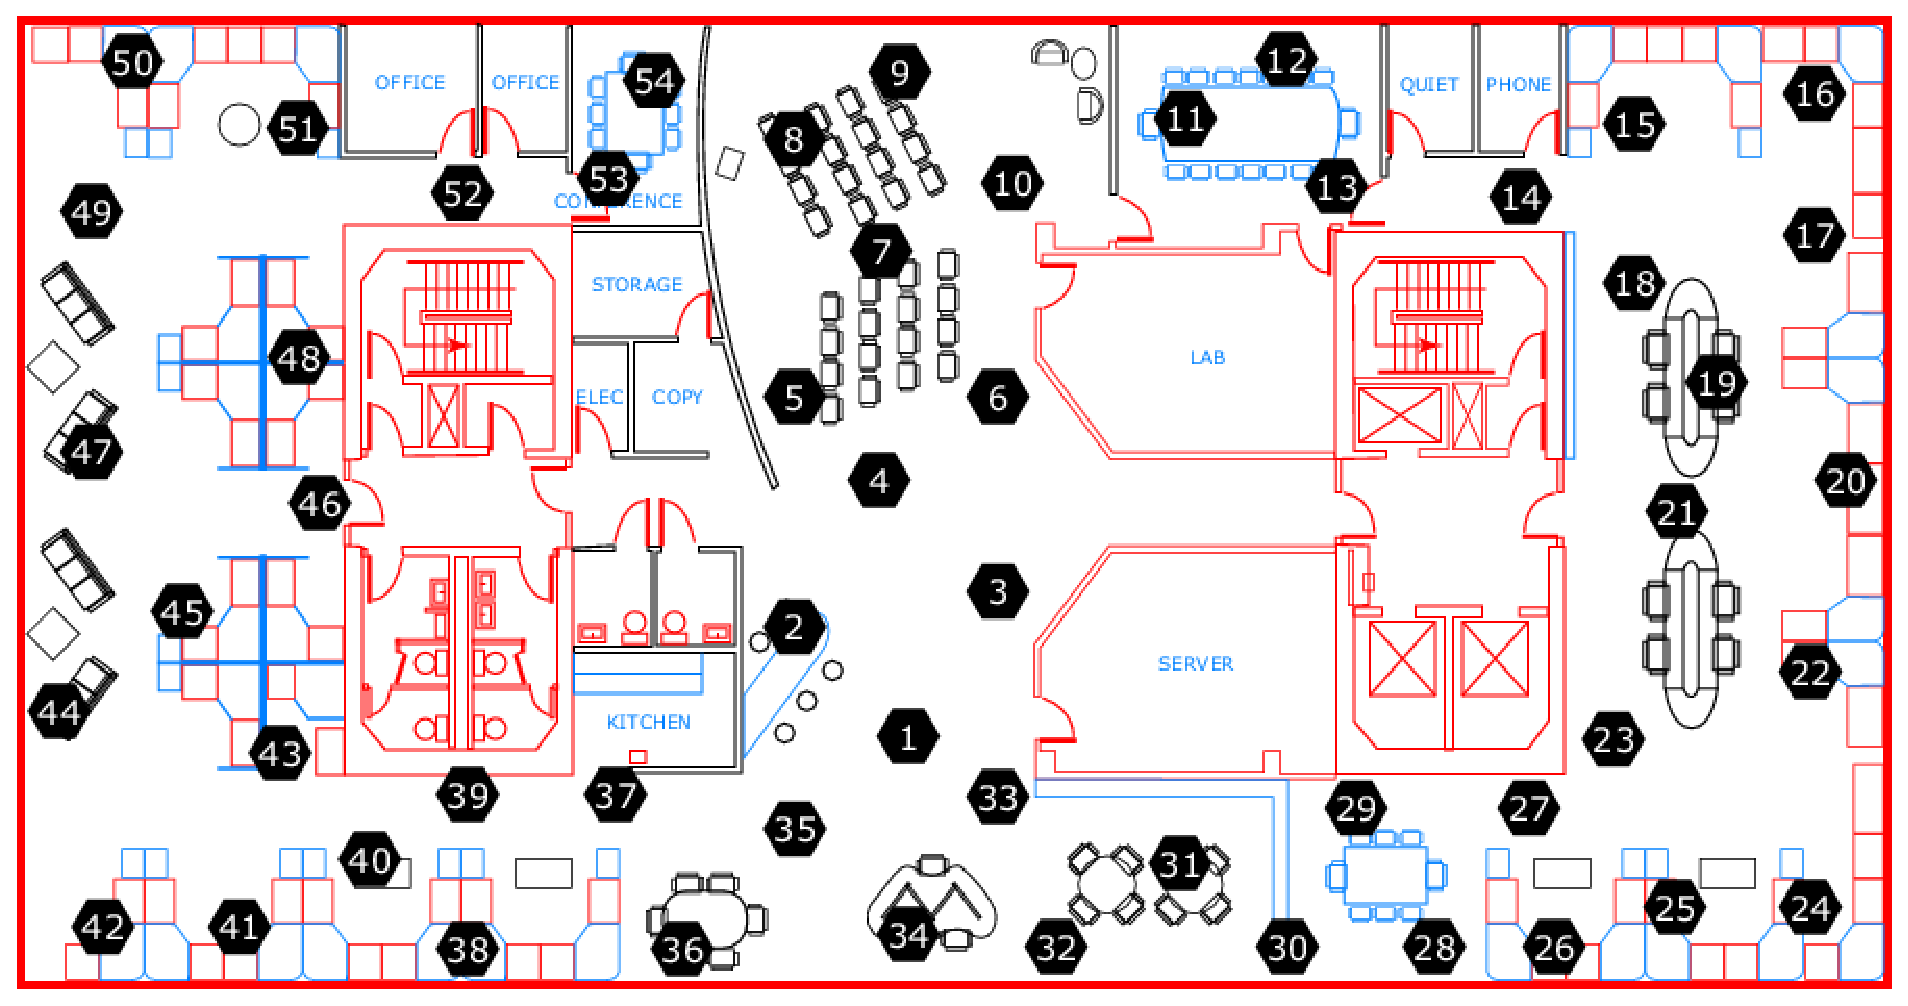
\includegraphics[height=2.5cm]{berkeley_lab.eps}
}
%\hspace{0.5cm}
\subfigure[\hbox{Traffic Sensor Deployment Map} \hbox{\hspace{0.5cm}(8 sensors of 20 shown)}]{
	\label{fig:traffic}
	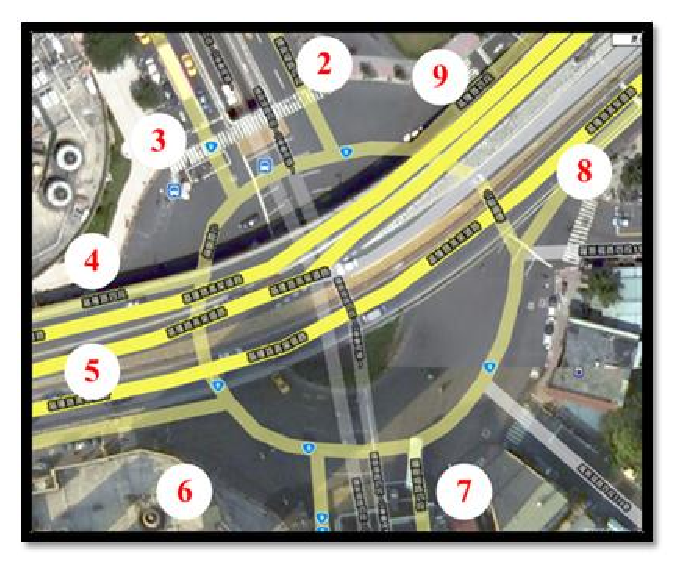
\includegraphics[height=2.5cm]{traffic_wsn.eps}
}
%\vspace{-0.3cm}
\end{figure}

%\vspace{-0.5cm}


%\subsubsection{Dataset Preparation}

%\paragraph{Berkeley Dataset Outlier Removal and Gridding}

%Gridding : Dataset falls on even 30s intervals for the first 5000 time steps (which is all we consider), so no additional gridding need be performed.
%Outlier Filtering : We use some simple rules to removed apparent errors. Observation removed if temperature \mbox{$>100\degc$}, temperature \mbox{$<5\degc$}, or humidity \mbox{$<16\%$}.

%\paragraph*{Traffic Dataset Outlier Removal and Gridding}


%Gridding : The original dataset recorded most readings at around the $xx:03$ and $xx:33$ minute marks, so a $6$ min window centered at these points captured the data for $30$ minute internal readings. Where more than one reading was recorded for a given node within a given window, the closest to the $3$ or $33$ minute mark was chosen. The full length of the dataset was used, which consists of $\approx 43$K 

%Outlier Filtering : Observation removed if temperature \mbox{$<5\degc$} or \mbox{$>60\degc$} or if humidity \mbox{$<10\%$} or \mbox{$>100\%$}.
\subsubsection{Missing Data Generation}

%Datasets of various lengths are produced from the single input dataset for our experiments, namely 2500, 5000, and 10000.
%There is an initially missing portion of the observations which can be considered Missing At Random (MAR).To this, we impose two different types of Missing Completely At Random (MCAR) sampling techniques to build validation and testing datasets.

Although both datasets intrinsically have missing readings, we cannot use those for evaluation because their true values are unknown.
Instead we devised two strategies to produce artificial missing data.
\paragraph*{Random Missing Pattern} ~
This pattern reflects repeatedly choosing a random time and random sensor to be missing and hence removed from the training set.
%
We define two variables $x$ and $y$ during our experiment, and the X-axis of the resulting plot varies with $x$.
\begin{itemize}
\item $10\%$ of the existing readings are randomly selected (without replacement) to be the validation set
\item $y\%$ of the existing readings are randomly selected (without replacement) to be the testing set
\item The remaining readings (x\%) are part of the training set. That is, x+y+10=100 that accounts for all the observed readings.
\end{itemize}

\paragraph*{Consecutive Missing Pattern} ~
This pattern reflects testing the effect of all data missing after a certain point in time.
We define two values $x$ and $y$ as follows.
\begin{itemize}
\item Here, we have the last $y\%$ of time covered as missing, and the prior $10\%$ to that is considered as the validation data.
\item The sensor node numbers ``covered up'' in the validation and testing for the Berkeley and traffic datasets are ${4,19,45}$ and ${2,4,6,8,10,14,17,19,20,21}$, respectively.
Note that node $21$ of the traffic dataset is the gateway node.
We experimented with other combinations of covered up nodes, and the results were similar.
\end{itemize}

\subsubsection{Parameter Setting}

We exploit the commonly used metric of root-mean-square-error (RMSE)
to measure the difference between the predicted values and the ground
truth, and all parameters in our models and competitors' models are
automatically selected using the validation set.

We share the resulting parameter values of our models.
The number of factors $K$ is $54$ for MF and $30$ for TF for the Berkeley dataset, and $21$ for MF and $10$ for TF for the traffic dataset. 
The learning rate $\eta$ is set to $0.04$ to $0.004$ for MF and $0.001$ to $0.0001$ for TF.
A smaller~$\eta$ or a larger~$K$ could slow down the training process, but it would not degrade 
the model.
Also, a reasonable choice of $K$ should not be larger than the number of sensor nodes since the rank of the matrix is at most $K$.
The temporal regularization $\gamma$ is set to $0.2/\eta$ in all of our experiments.
The conventional regularization $\beta$ is $0.001$ for consecutive missing and $0$ for random missing in MF, 
while in TF, $\beta$ is $0.005$ for consecutive missing and $0.001$ for random missing.

\subsection{Experimental Results on TR-MF} \label{subsec:exp_basic}%from Chung-Yi
We compare our TR-MF with conventional MF (i.e. MF without temporal regularization), Linear Interpolation~(LI), Applying K-nearest neighbour Estimation~(AKE), Data Estimation using Statistical Model~(DESM), Spatial temporal imputation~(STI) and Multiple Inputation (MI).
%We implemented AKE, DESM, STI, and for MI we use the EM-imputation from LISREL.  
Note that we only know the location information of 8 out of 20 sensors in traffic data set, but the pairwise distance values are mandatary to execute DESM and STI. For them, we simply assume the distances are all equal.

%validation setting
%Table \ref{table:berkeley_random_hum}, \ref{table:berkeley_random_light} and \ref{table:berkeley_random_tem} show the results of different models random split on Berkeley data set. In the plot, the x-axis represents the missing ratio. Conceivably the difficulty of an imputation task arises with th increase of missing ratio, therefore we can see that the slopes for most of the lines in the plot are nonpositive. Also note that to highlight the difference between the better models, we cut the overflowed RMSE values of the inferior models to the maximum values that can be displayed in the plot. That says, the flat lines on top of the plots usually indicate the exact RMSE is even higher than what has been shown.

Figure \ref{fig:berkeley_random_hum}, \ref{fig:berkeley_random_light}, \ref{fig:berkeley_random_tem}, \ref{fig:traffic_random_hum} and \ref{fig:traffic_random_tem} show the result of random missing. The outcome indicates several interesting facts. First, TR-MF outperforms the original MF significantly, which demonstrates the effectiveness of the temporal regularization. In general, TR-MF shows significant improvement over all the other methods. On the other hand, LT is quite competitive on Berkeley data, especially for lower missing ratio cases. This is because the sampling rate of Berkeley data set is fairly high, so using only temporal correlation is sufficient to obtain decent results. In a data set with lower sampling rate as the traffic data, the spatial-oriented methods such as AKE outperform LI. 

%\begin{table}[htbp]
%\setlength{\tabcolsep}{2pt}
%\centering
%\caption{RMSE of (Berkeley, random, humidity)}
%\label{table:berkeley_random_hum}
%\begin{tabular}{ r | r r r r r r}
%	train	&LI	&TR-MF	&AKE	&DESM	&STI &MI\\ \hline
%	10\% & $ 0.171_{(2)} $ & $ \mathbf{ 0.142_{(1)} } $ & $ 0.264_{(3)} $ & $ 0.544_{(4)} $ & $ 1.220_{(5)} $&$0.190$ \\
%	20\% & $ 0.127_{(2)} $ & $ \mathbf{ 0.114_{(1)} } $ & $ 0.244_{(3)} $ & $ 0.318_{(4)} $ & $ 1.472_{(5)} $ &$ 0.151$\\
%	40\% & $ 0.095_{(2)} $ & $ \mathbf{ 0.092_{(1)} } $ & $ 0.199_{(3)} $ & $ 0.219_{(4)} $ & $ 1.648_{(5)} $ &$ 0.101$\\
%	60\% & $ 0.085_{(2)} $ & $ \mathbf{ 0.082_{(1)} } $ & $ 0.181_{(4)} $ & $ 0.180_{(3)} $ & $ 1.649_{(5)} $ &$ 0.092$\\
%	80\% & $ \mathbf{ 0.075_{(1)} } $ & $ 0.076_{(2)} $ & $ 0.127_{(3)} $ & $ 0.160_{(4)} $ & $ 1.604_{(5)} $ &$0.079$ \\
%	85\% & $ \mathbf{ 0.074_{(1)} } $ & $ 0.075_{(2)} $ & $ 0.121_{(3)} $ & $ 0.148_{(4)} $ & $ 1.549_{(5)} $ &$0.082$ \\ \hline
%	rank &1.67 &1.33 &3.17 &3.83 &5.00 \\
%\end{tabular}
%\end{table}
%
%\begin{table} [htbp]
%\setlength{\tabcolsep}{2pt}
%\centering
%\caption{RMSE of (Berkeley, random, light)}
%\label{table:berkeley_random_light}
%\begin{tabular}{ r |  r r r r r r}
%	train	&LI	&TR-MF	&AKE	&DESM	&STI &MI\\ \hline
%	10\% & $ 52.9_{(2)} $ & $ \mathbf{ 35.5_{(1)} } $ & $ 61.2_{(3)} $ & $ 6250.4_{(5)} $ & $ 258.2_{(4)} $ &$103.3$ \\
%	20\% & $ 38.7_{(2)} $ & $ \mathbf{ 28.2_{(1)} } $ & $ 53.0_{(3)} $ & $ 215.9_{(4)} $ & $ 311.0_{(5)} $ &$70.3$\\
%	40\% & $ 29.9_{(2)} $ & $ \mathbf{ 21.2_{(1)} } $ & $ 41.4_{(3)} $ & $ 356.7_{(5)} $ & $ 356.3_{(4)} $ &$48.2$\\
%	60\% & $ 25.0_{(2)} $ & $ \mathbf{ 17.2_{(1)} } $ & $ 33.7_{(3)} $ & $ 112.6_{(4)} $ & $ 366.9_{(5)} $ &$39.9$\\
%	80\% & $ 23.9_{(2)} $ & $ \mathbf{ 17.7_{(1)} } $ & $ 27.9_{(3)} $ & $ 41.7_{(4)} $ & $ 363.3_{(5)} $ &$42.1$\\
%	85\% & $ 20.9_{(2)} $ & $ \mathbf{ 14.4_{(1)} } $ & $ 24.3_{(3)} $ & $ 44.4_{(4)} $ & $ 354.2_{(5)} $ &$29.3$\\ \hline
%	rank &2.00 &1.00 &3.00 &4.33 &4.67 \\
%\end{tabular}
%\end{table}
%
%\begin{table}[htbp]
%\setlength{\tabcolsep}{2pt}
%\centering
%\caption{RMSE of (Berkeley, random, temperature)}
%\label{table:berkeley_random_tem}
%\begin{tabular}{ r | r r r r r r}
%	train	&LI	&TR-MF	&AKE	&DESM	&STI &MI\\ \hline
%	10\% & $ 0.070_{(2)} $ & $ \mathbf{ 0.046_{(1)} } $ & $ 0.112_{(3)} $ & $ 0.298_{(4)} $ & $ 0.506_{(5)} $ &$0.121$\\
%	20\% & $ 0.042_{(2)} $ & $ \mathbf{ 0.032_{(1)} } $ & $ 0.111_{(3)} $ & $ 0.167_{(4)} $ & $ 0.584_{(5)} $ &$0.098$\\
%	40\% & $ 0.027_{(2)} $ & $ \mathbf{ 0.023_{(1)} } $ & $ 0.080_{(3)} $ & $ 0.095_{(4)} $ & $ 0.644_{(5)} $ &$0.094$\\
%	60\% & $ 0.021_{(2)} $ & $ \mathbf{ 0.018_{(1)} } $ & $ 0.053_{(3)} $ & $ 0.067_{(4)} $ & $ 0.637_{(5)} $ &$0.091$\\
%	80\% & $ 0.016_{(2)} $ & $ \mathbf{ 0.015_{(1)} } $ & $ 0.043_{(3)} $ & $ 0.048_{(4)} $ & $ 0.611_{(5)} $ &$0.078$\\
%	85\% & $ 0.019_{(2)} $ & $ \mathbf{ 0.016_{(1)} } $ & $ 0.034_{(3)} $ & $ 0.048_{(4)} $ & $ 0.593_{(5)} $ &$0.082$\\ \hline
%	rank &2.00 &1.00 &3.00 &4.00 &5.00 \\
%\end{tabular}
%\end{table}


%\begin{table} [htbp]
%\setlength{\tabcolsep}{2pt}
%\centering
%\caption{RMSE of (traffic, random, humidity)}
%\label{table:traffic_random_hum}
%\begin{tabular}{ r | r r r r r r}
%	train	&LI	&TR-MF	&AKE	&DESM	&STI &MI\\ \hline
%	10\% & $ 11.630_{(4)} $ & $ \mathbf{ 3.524_{(1)} } $ & $ 7.307_{(2)} $ & $ 19.817_{(5)} $ & $ 10.625_{(3)} $ & $4.708$  \\
%	20\% & $ 7.269_{(4)} $ & $ \mathbf{ 2.583_{(1)} } $ & $ 4.559_{(2)} $ & $ 14.634_{(5)} $ & $ 6.745_{(3)}  $    & $4.304$\\
%	40\% & $ 4.233_{(3)} $ & $ \mathbf{ 1.932_{(1)} } $ & $ 3.458_{(2)} $ & $ 8.986_{(5)} $ & $ 5.021_{(4)} $       & $3.794$\\
%	60\% & $ 3.184_{(3)} $ & $ \mathbf{ 1.664_{(1)} } $ & $ 2.901_{(2)} $ & $ 6.396_{(5)} $ & $ 4.710_{(4)} $       & $3.502$\\
%	80\% & $ 2.690_{(3)} $ & $ \mathbf{ 1.565_{(1)} } $ & $ 2.511_{(2)} $ & $ 4.714_{(5)} $ & $ 4.605_{(4)} $       &$3.284$\\
%	85\% & $ 2.588_{(3)} $ & $ \mathbf{ 1.503_{(1)} } $ & $ 2.401_{(2)} $ & $ 4.382_{(4)} $ & $ 4.671_{(5)} $       & $3.308$\\ \hline
%	rank &3.33 &1.00 &2.00 &4.83 &3.83 \\
%\end{tabular}
%\end{table}
%
%\begin{table} [htbp]
%\setlength{\tabcolsep}{2pt}
%\centering
%\caption{RMSE of (traffic, random, temperature)}
%\label{table:traffic_random_tem}
%\begin{tabular}{ r | r r r r r r}
%	train	&LI	&TR-MF	&AKE	&DESM	&STI  &MI\\ \hline
%	10\% & $ 4.000_{(4)} $ & $ \mathbf{ 1.214_{(1)} } $ & $ 2.509_{(2)} $ & $ 6.212_{(5)} $ & $ 3.662_{(3)} $ &$1.541$\\
%	20\% & $ 2.508_{(4)} $ & $ \mathbf{ 0.898_{(1)} } $ & $ 1.538_{(2)} $ & $ 4.867_{(5)} $ & $ 2.261_{(3)} $ &$1.426$\\
%	40\% & $ 1.477_{(3)} $ & $ \mathbf{ 0.689_{(1)} } $ & $ 1.192_{(2)} $ & $ 3.149_{(5)} $ & $ 1.732_{(4)} $ &$1.281$\\
%	60\% & $ 1.101_{(3)} $ & $ \mathbf{ 0.585_{(1)} } $ & $ 1.005_{(2)} $ & $ 2.275_{(5)} $ & $ 1.597_{(4)} $ &$1.213$\\
%	80\% & $ 0.938_{(3)} $ & $ \mathbf{ 0.551_{(1)} } $ & $ 0.885_{(2)} $ & $ 1.702_{(5)} $ & $ 1.574_{(4)} $ &$1.117$\\
%	85\% & $ 0.915_{(3)} $ & $ \mathbf{ 0.519_{(1)} } $ & $ 0.866_{(2)} $ & $ 1.494_{(4)} $ & $ 1.585_{(5)} $& $1.102$\\ \hline
%	rank &3.33 &1.00 &2.00 &4.83 &3.83 \\
%\end{tabular}
%\end{table}

%\subsubsection{Consecutive Missing Pattern}
%Table \ref{table:berkeley_temporal_hum}, \ref{table:berkeley_temporal_light} and \ref{table:berkeley_temporal_tem} show the result for Consecutive Missing Pattern on Berkeley data set and Table \ref{table:traffic_temporal_hum} and \ref{table:traffic_temporal_tem} on traffic data set.
Figure \ref{fig:berkeley_temporal_hum}, \ref{fig:berkeley_temporal_light}, \ref{fig:berkeley_temporal_tem} and \ref{fig:traffic_temporal_hum} and \ref{fig:traffic_temporal_tem} show the result of consecutive missing pattern. Comparing it with the previous figure, we can find that the consecutive missing task is more challenging as the RMSE is much higher than that of random missing.
Generally speaking, the temporal correlation is not very useful in consecutive missing cases. Thus, linear inpolation is no longer competitive and the performance between TR-MF and MF has become closer, in particular when the missing ratio is high. The AKE algorithm also performs competitively. The results indicate that when there are less information a model can learn from in temporal dimension, providing it other kinds of information (e.g. the spatial information ) can potentially improve the outcomes. Such hypothesize is confirmed in the next experiment which shows that TR-MF can be further improved in consecutive missing cases if the spatial information is included. 


%\begin{table}[htbp]
%\setlength{\tabcolsep}{2pt}
%\centering
%\caption{RMSE of (Berkeley, temporal, humidity)}
%\label{table:berkeley_temporal_hum}
%\begin{tabular}{ r | r r r r r r}
%	train	&LI	&TR-MF	&AKE	&DESM	&STI &MI\\ \hline
%	10\% & $ 4.183_{(4)} $ & $ 0.957_{(2)} $ & $ 1.669_{(3)} $ & $ 4.185_{(5)} $ & $ \mathbf{ 0.792_{(1)} } $&$2.710$  \\
%	20\% & $ 5.421_{(4)} $ & $ \mathbf{ 0.796_{(1)} } $ & $ 0.969_{(3)} $ & $ 5.422_{(5)} $ & $ 0.865_{(2)} $ &$2.193$ \\
%	40\% & $ 6.443_{(4)} $ & $ \mathbf{ 0.771_{(1)} } $ & $ 1.025_{(3)} $ & $ 6.443_{(5)} $ & $ 0.961_{(2)} $ &$1.629$ \\
%	60\% & $ 2.223_{(4)} $ & $ \mathbf{ 0.540_{(1)} } $ & $ 0.928_{(3)} $ & $ 2.233_{(5)} $ & $ 0.864_{(2)} $ &$1.284$ \\
%	80\% & $ 1.208_{(4)} $ & $ \mathbf{ 0.447_{(1)} } $ & $ 0.636_{(2)} $ & $ 1.216_{(5)} $ & $ 0.688_{(3)} $ &$1.171$  \\
%	85\% & $ 2.306_{(4)} $ & $ \mathbf{ 0.323_{(1)} } $ & $ 0.777_{(2)} $ & $ 2.308_{(5)} $ & $ 0.796_{(3)} $ &$0.966$ \\ \hline
%	rank &4.00 &1.17 &2.67 &5.00 &2.17 \\
%\end{tabular}
%\end{table}
%
%\begin{table}[htbp]
%\setlength{\tabcolsep}{2pt}
%\centering
%\caption{RMSE of (Berkeley, temporal, light)}
%\label{table:berkeley_temporal_light}
%\begin{tabular}{ r | r r r r r r}
%	train	&LI	&TR-MF	&AKE	&DESM	&STI &MI\\ \hline
%	10\% & $ 320.0_{(5)} $ & $ \mathbf{ 220.1_{(1)} } $ & $ 239.1_{(2)} $ & $ 320.0_{(4)} $ & $ 251.3_{(3)} $ &$331.2$ \\
%	20\% & $ 497.8_{(4)} $ & $ \mathbf{ 113.3_{(1)} } $ & $ 257.1_{(3)} $ & $ 499.7_{(5)} $ & $ 206.6_{(2)} $ &$412.7$\\
%	40\% & $ 194.5_{(3)} $ & $ \mathbf{ 58.1_{(1)} } $ & $ 68.5_{(2)} $ & $ 195.2_{(4)} $ & $ 208.3_{(5)} $ &$99.6$\\
%	60\% & $ 312.1_{(4)} $ & $ \mathbf{ 41.7_{(1)} } $ & $ 77.5_{(2)} $ & $ 312.1_{(5)} $ & $ 289.2_{(3)} $ &$153.6$\\
%	80\% & $ 293.5_{(4)} $ & $ \mathbf{ 21.4_{(1)} } $ & $ 84.9_{(2)} $ & $ 293.9_{(5)} $ & $ 213.9_{(3)} $ &$201.3$\\
%	85\% & $ 277.9_{(4)} $ & $ \mathbf{ 8.3_{(1)} } $ & $ 79.0_{(2)} $ & $ 280.4_{(5)} $ & $ 92.7_{(3)} $ &$198.4$\\ \hline
%	rank &4.00 &1.00 &2.17 &4.67 &3.17 \\
%\end{tabular}
%\end{table}
%
%
%
%\begin{table}[htbp]
%\setlength{\tabcolsep}{2pt}
%\centering
%\caption{RMSE of (Berkeley, temporal, temperature)}
%\label{table:berkeley_temporal_tem}
%\begin{tabular}{ r | r r r r r r}
%    10\% & $ 3.760_{(4)} $ & $ 0.515_{(3)} $ & $ 0.514_{(2)} $ & $3.761_{(5)}$ & $\mathbf{ 0.492_{(1)}}$ &$1.712$\\
%    20\% & $ 2.320_{(4)} $ & $ \mathbf{ 0.392_{(1)} } $ & $ 0.406_{(2)} $ & $ 2.321_{(5)} $ & $ 0.415_{(3)} $ &$1.985$\\
%    40\% & $ 3.595_{(4)} $ & $ 0.310_{(2)} $ & $ \mathbf{ 0.304_{(1)} } $ & $ 3.595_{(5)} $ & $ 0.486_{(3)} $ &$1.788$\\
%    60\% & $ 1.960_{(4)} $ & $ \mathbf{ 0.206_{(1)} } $ & $ 0.340_{(2)} $ & $ 1.962_{(5)} $ & $ 0.532_{(3)} $ &$1.541$\\
%    80\% & $ 0.887_{(4)} $ & $ \mathbf{ 0.132_{(1)} } $ & $ 0.280_{(2)} $ & $ 0.894_{(5)} $ & $ 0.326_{(3)} $ &$0.971$\\
%    85\% & $ 1.024_{(5)} $ & $ \mathbf{ 0.088_{(1)} } $ & $ 0.305_{(2)} $ & $ 1.016_{(4)} $ & $ 0.351_{(3)} $ &$0.644$\\ \hline
%rank &4.17 &1.50 &1.83 &4.83 &2.67 \\
%\end{tabular}
%\end{table}


%\begin{table} [htbp]
%\setlength{\tabcolsep}{2pt}
%\centering
%\caption{RMSE of (traffic, temporal, humidity)}
%\label{table:traffic_temporal_hum}
%\begin{tabular}{ r | r r r r r r}
%	train	&LI	&TR-MF	&AKE	&DESM	&STI &MI\\ \hline
%	10\% & $ 27.751_{(4)} $ & $ 5.195_{(2)} $ & $ \mathbf{ 5.081_{(1)} } $ & $ 27.794_{(5)} $ & $ 5.752_{(3)} $ &$5.920$\\
%	20\% & $ 21.469_{(4)} $ & $ 5.487_{(2)} $ & $ \mathbf{ 5.020_{(1)} } $ & $ 22.372_{(5)} $ & $ 5.641_{(3)} $ &$5.504$\\
%	40\% & $ 25.828_{(4)} $ & $ 5.782_{(2)} $ & $ \mathbf{ 5.193_{(1)} } $ & $ 25.997_{(5)} $ & $ 5.957_{(3)} $ &$5.905$\\
%	60\% & $ 27.489_{(4)} $ & $ \mathbf{ 4.954_{(1)} } $ & $ 5.027_{(2)} $ & $ 27.517_{(5)} $ & $ 6.372_{(3)} $ &$5.457$\\
%	80\% & $ 18.936_{(4)} $ & $ 4.564_{(2)} $ & $ \mathbf{ 4.194_{(1)} } $ & $ 19.398_{(5)} $ & $ 4.972_{(3)} $ &$4.789$\\
%	85\% & $ 23.513_{(4)} $ & $ 4.248_{(2)} $ & $ \mathbf{ 3.666_{(1)} } $ & $ 23.615_{(5)} $ & $ 4.695_{(3)} $ &$5.064$\\ \hline
%	rank &4.00 &1.83 &1.17 &5.00 &3.00 \\
%\end{tabular}
%\end{table}


%\begin{table} [htbp]
%\setlength{\tabcolsep}{2pt}
%\centering
%\caption{RMSE of (traffic, temporal, temperture)}
%\label{table:traffic_temporal_tem}
%\begin{tabular}{ r | r r r r r r}
%	train	&LI	&TR-MF	&AKE	&DESM	&STI &MI\\ \hline
%	10\% & $ 11.435_{(4)} $ & $ 1.700_{(2)} $ & $ \mathbf{ 1.679_{(1)} } $ & $ 11.551_{(5)} $ & $ 2.089_{(3)} $ &$1.785$\\
%	20\% & $ 7.186_{(4)} $ & $ 1.812_{(2)} $ & $ \mathbf{ 1.664_{(1)} } $ & $ 7.259_{(5)} $ & $ 1.956_{(3)} $ &$1.765$\\
%	40\% & $ 10.594_{(4)} $ & $ 1.832_{(2)} $ & $ \mathbf{ 1.579_{(1)} } $ & $ 10.639_{(5)} $ & $ 2.048_{(3)} $& $1.724$\\
%	60\% & $ 14.134_{(4)} $ & $ \mathbf{ 1.666_{(1)} } $ & $ 1.687_{(2)} $ & $ 14.251_{(5)} $ & $ 2.780_{(3)} $ &$1.712$\\
%	80\% & $ 16.166_{(5)} $ & $ 1.430_{(2)} $ & $ \mathbf{ 1.414_{(1)} } $ & $ 16.139_{(4)} $ & $ 1.710_{(3)} $ &$1.594$\\
%	85\% & $ 10.022_{(5)} $ & $ 1.441_{(2)} $ & $ \mathbf{ 1.356_{(1)} } $ & $ 9.992_{(4)} $ & $ 1.719_{(3)} $ &$1.389$\\ \hline
%	rank &4.33 &1.83 &1.17 &4.67 &3.00 \\
%\end{tabular}
%\end{table}



%\begin{figure}[H]
%\centering
%\input{table11.pspdftex}
%\caption{RMSE of (traffic, temporal, temperature); LI and DESM not shown as RMSE is greater than 7}
%\end{figure}
%
%
%\begin{figure*}[ht]
%\centering
%
%\subfigure[subFig 1 caption]{
%	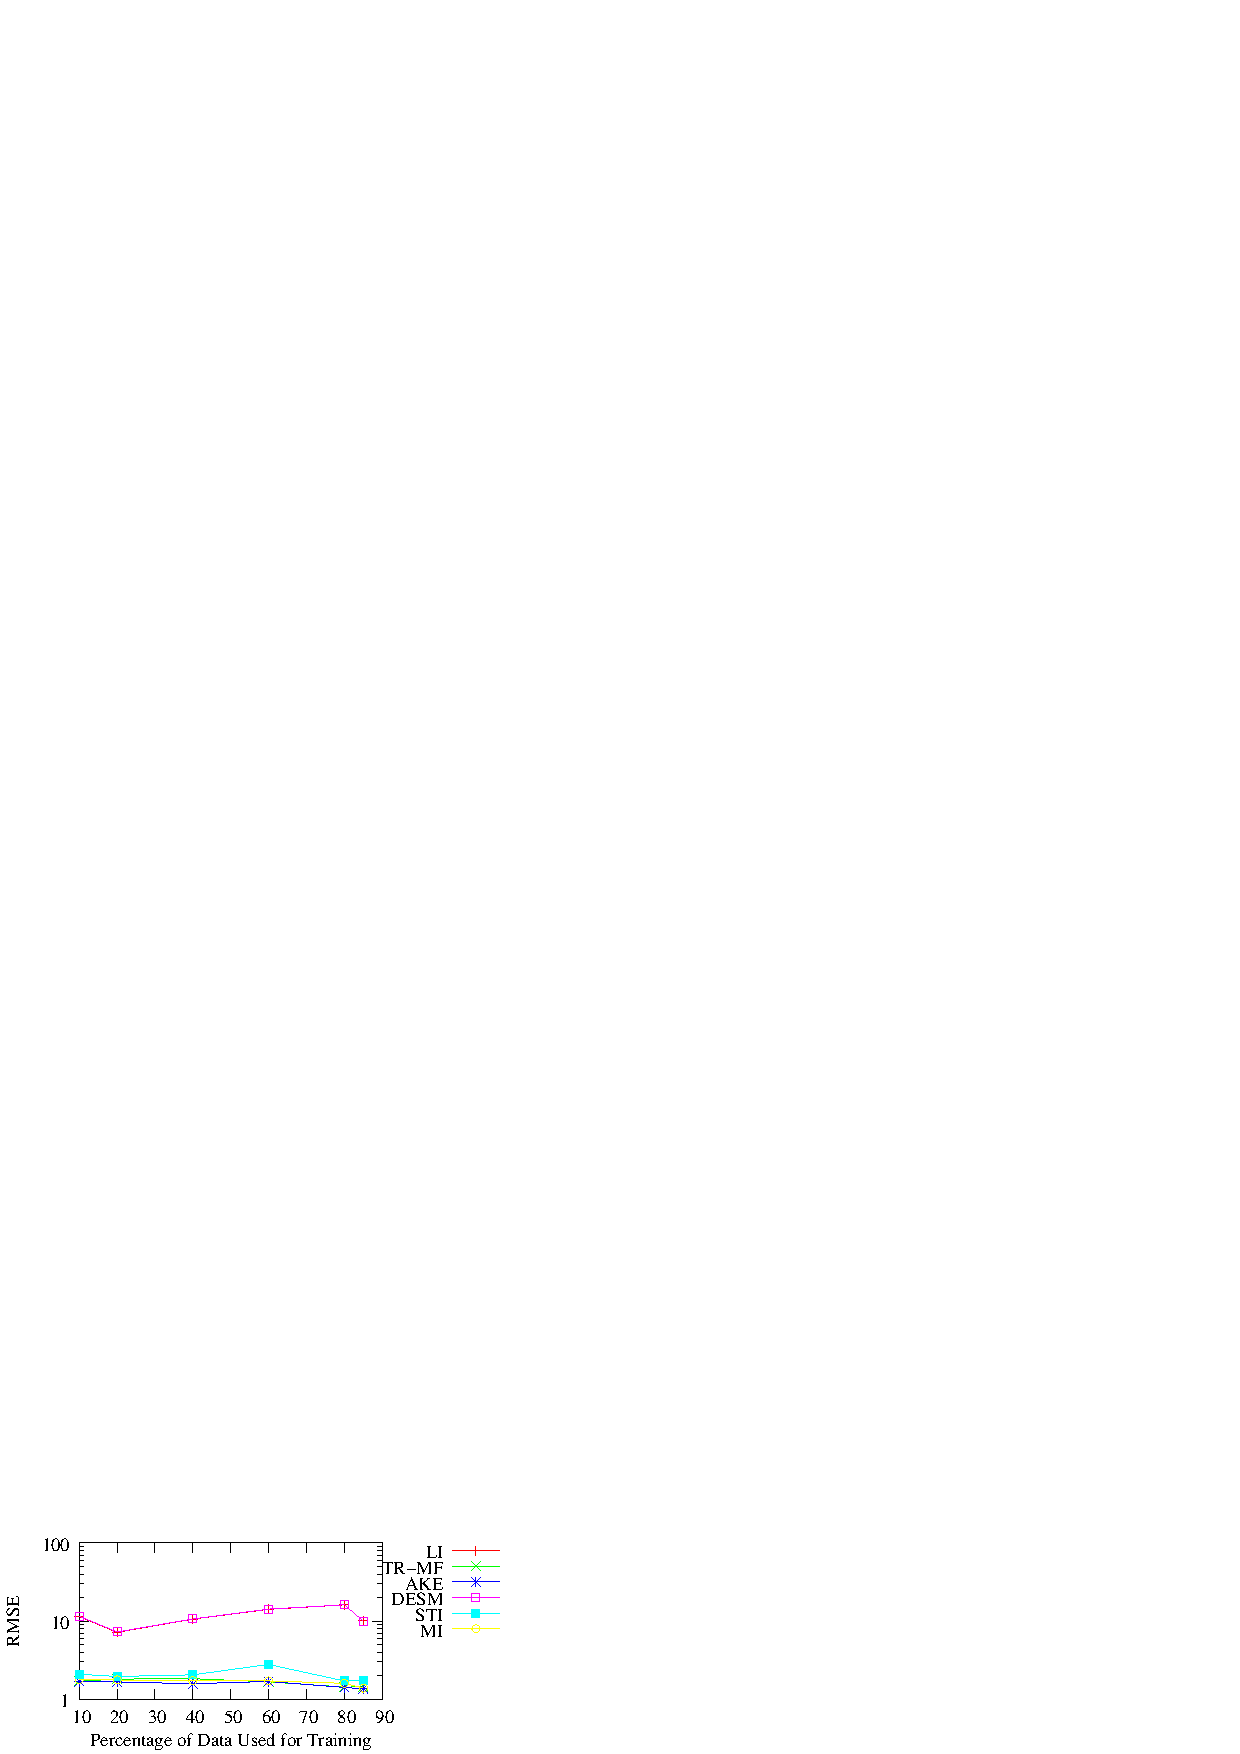
\includegraphics[width=0.45\textwidth]{table11_pspdftex.pdf}
%	\label{fig: 1}
%}
%\hspace{0in}
%\subfigure[subFig 2 caption]{
%	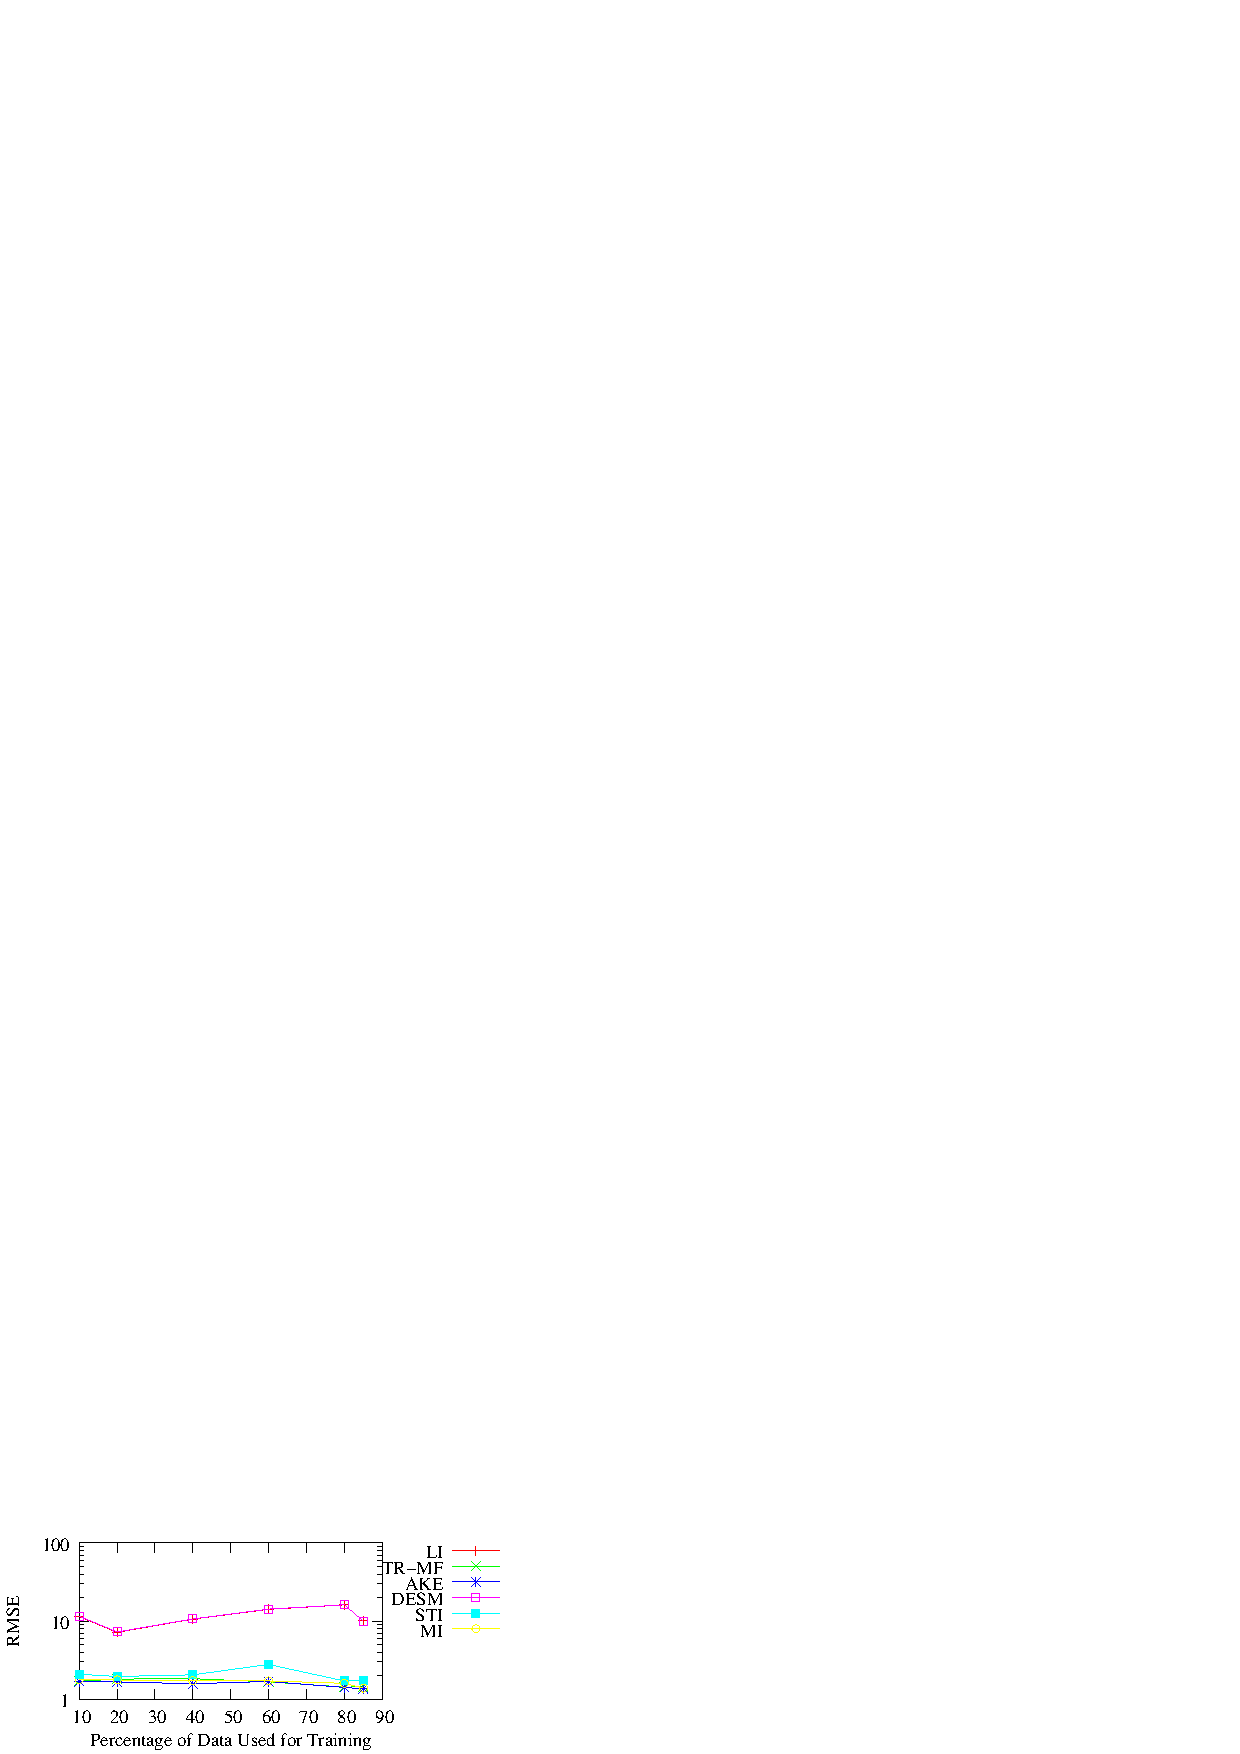
\includegraphics[width=0.45\textwidth]{table11_pspdftex.pdf}
%	\label{fig: 2}
%}
%
%\caption[nanana]{Global caption}
%\end{figure*}

\subsection{Results on STR-MF} \label{experimental_results_spatial}
Since

Table \ref{table:spatial_random_hum}, \ref{table:spatial_random_light}, \ref{table:spatial_random_tem}, \ref{table:spatial_temporal_hum}, \ref{table:spatial_temporal_light}, \ref{table:spatial_temporal_tem}  show the result of adding spatial regularization. 
STR-MF mean TR-MF with strong spatial regularization, while sTR-MF is with weak spatial regularization.

We got no improvement after adding spatial regularization on random split and light 
. This is because TR-MF already learns the spatial correlation from the data: we will get similar factors for correlated sensor nodeg. 

\begin{table} [htbp]
\setlength{\tabcolsep}{2pt}
\centering
\small
\begin{tabular} {c | r r r | r r r | r r r}
& \multicolumn{3}{ c|}{Humidity} & \multicolumn{3}{|c|}{Light} & \multicolumn{3}{|c }{Temperature} \\ \hline
train & \begin{turn}{65}TR-MF\end{turn} & \begin{turn}{65}STR-MF\end{turn} & \begin{turn}{65}sTR-MF\end{turn}& \begin{turn}{65}TR-MF\end{turn} & \begin{turn}{65}STR-MF\end{turn} & \begin{turn}{65}sTR-MF\end{turn}& \begin{turn}{65}TR-MF\end{turn} & \begin{turn}{65}STR-MF\end{turn} & \begin{turn}{65}sTR-MF\end{turn} \\ \hline
10\% & $ \mathbf{ 0.142 } $ & $ 0.484 $ & $ 0.173 $ & $ \mathbf{ 35.5 } $ & $ 97.4 $ & $ 38.3 $ & $ \mathbf{ 0.046 } $ & $ 0.154 $ & $ 0.061 $\\
20\% & $ \mathbf{ 0.114 } $ & $ 0.424 $ & $ 0.135 $ & $ \mathbf{ 28.2 } $ & $ 90.6 $ & $ 28.9 $ & $ \mathbf{ 0.032 } $ & $ 0.146 $ & $ 0.047 $\\
40\% & $ \mathbf{ 0.092 } $ & $ 0.352 $ & $ 0.104 $ & $ \mathbf{ 21.2 } $ & $ 85.8 $ & $ 22.8 $ & $ \mathbf{ 0.023 } $ & $ 0.145 $ & $ 0.037 $\\
60\% & $ \mathbf{ 0.082 } $ & $ 0.337 $ & $ 0.093 $ & $ \mathbf{ 17.2 } $ & $ 83.3 $ & $ 18.3 $ & $ \mathbf{ 0.018 } $ & $ 0.147 $ & $ 0.031 $\\
80\% & $ \mathbf{ 0.076 } $ & $ 0.324 $ & $ 0.084 $ & $ \mathbf{ 17.7 } $ & $ 84.4 $ & $ 18.1 $ & $ \mathbf{ 0.015 } $ & $ 0.148 $ & $ 0.027 $\\
85\% & $ \mathbf{ 0.075 } $ & $ 0.326 $ & $ 0.083 $ & $ \mathbf{ 14.4 } $ & $ 82.0 $ & $ 15.8 $ & $ \mathbf{ 0.016 } $ & $ 0.138 $ & $ 0.028 $\\
\end{tabular}
\caption{RMSE of Berkeley Random split} \label{table:spatial_random}
\end{table}

\begin{table} [htbp]
\setlength{\tabcolsep}{2pt}
\centering
\small
\begin{tabular} {c | r r r | r r r | r r r}
& \multicolumn{3}{ c|}{Humidity} & \multicolumn{3}{|c|}{Light} & \multicolumn{3}{|c }{Temperature} \\ \hline
train & \begin{turn}{65}TR-MF\end{turn} & \begin{turn}{65}STR-MF\end{turn} & \begin{turn}{65}sTR-MF\end{turn}& \begin{turn}{65}TR-MF\end{turn} & \begin{turn}{65}STR-MF\end{turn} & \begin{turn}{65}sTR-MF\end{turn}& \begin{turn}{65}TR-MF\end{turn} & \begin{turn}{65}STR-MF\end{turn} & \begin{turn}{65}sTR-MF\end{turn} \\ \hline
10\% & $ 0.957 $&$ 0.573 $&$ \mathbf{ 0.547 } $&$ \mathbf{ 220.070 } $&$ 281.607 $&$ 264.763 $&$ 0.515 $&$ \mathbf{ 0.242 } $&$ 0.307 $\\
20\% & $ 0.796 $&$ 0.657 $&$ \mathbf{ 0.459 } $&$ \mathbf{ 113.310 } $&$ 236.865 $&$ 230.054 $&$ 0.392 $&$ \mathbf{ 0.179 } $&$ 0.187 $\\
40\% & $ 0.771 $&$ 0.520 $&$ \mathbf{ 0.455 } $&$ \mathbf{ 58.090 } $  & $ 110.758 $ &  $ 64.388 $&$ 0.310 $&$ 0.196 $&$ \mathbf{ 0.189 } $\\
60\% & $ 0.540 $&$ \mathbf{ 0.351 } $&$ 0.708 $&$ \mathbf{ 41.730 } $  & $ 150.149 $ &  $ 69.235 $&$ 0.206 $&$ \mathbf{ 0.191 } $&$ 0.243 $\\
80\% & $ 0.447 $&$ 0.299 $&$ \mathbf{ 0.261 } $&$ \mathbf{ 21.450 } $  & $ 112.694 $ &  $ 28.017 $&$ 0.132 $&$ \mathbf{ 0.108 } $&$ 0.114 $\\
85\% & $ 0.323 $&$ \mathbf{ 0.166 } $&$ 0.256 $&$ \mathbf{ 8.310 } $   & $ 85.423 $  &  $ 12.079 $&$ 0.088 $&$ \mathbf{ 0.065 } $&$ 0.082 $\\
\end{tabular}
\caption{RMSE of Berkeley Temporal split} \label{table:spatial_temporal}
\end{table}


\subsection{Multivariate Learning}
\subsubsection{Multivariate TRMF}

\begin{table}[htbp]
\caption{Multivariate RMSE (Berkeley, random)}
\label{traffic}
\begin{tabular}{r | r r r}
	&TRMF	&MtMF-Train	&MtMF-all \\ \hline
humid10-10-80	&0.1424	&0.1420	&0.1222\\
humid20-10-70	&0.1135	&0.1135	&0.0973\\
humid40-10-50	&0.0916	&0.0909	&0.0822\\
humid60-10-30	&0.0817	&0.0806	&0.0758\\
humid80-10-10	&0.0757	&0.0748	&0.0709\\
humid85-10- 5	&0.0751	&0.0739	&0.0712\\
 temp10-10-80	&0.1137	&0.1148	&0.0729\\
 temp20-10-70	&0.0462	&0.0481	&0.0369\\
 temp40-10-50	&0.0316	&0.0328	&0.0263\\
 temp60-10-30	&0.023	&0.0232	&0.0201\\
 temp80-10-10	&0.0182	&0.0183	&0.0166\\
 temp85-10- 5	&0.0153	&0.0154	&0.0143\\
\end{tabular}
\end{table}


\begin{table}[htbp]
\caption{Multivariate RMSE (Berkeley, temporal)}
\label{traffic}
\begin{tabular}{r | r r r}
	&TRMF	&MtMF-Train	&MtMF-all \\ \hline
humid10-10-80t	&0.957&0.996& 	0.991\\
humid20-10-70t	&0.796&0.852& 	0.846\\
humid40-10-50t	&0.771&0.835& 	0.807\\
humid60-10-30t	&0.540&0.887& 	0.880\\
humid80-10-10t	&0.447&0.483& 	0.480\\
humid85-10- 5t	&0.323&0.356& 	0.348\\
 temp10-10-80t	&0.515&0.567& 	0.555\\
 temp20-10-70t	&0.392&0.491& 	0.485\\
 temp40-10-50t	&0.310&0.380& 	0.347\\
 temp60-10-30t	&0.206&0.309& 	0.257\\
 temp80-10-10t	&0.132&0.429& 	0.432\\
 temp85-10- 5t	&0.088&0.122& 	0.114\\
\end{tabular}
\end{table}

\begin{table}[htbp]
\caption{Multivariate RMSE (traffic Data, Random)}
\label{traffic}
\begin{tabular}{r | r r r}
	&TRMF	&MtMF-Train	&MtMF-all \\ \hline
humid10-10-80	&3.524 	&3.486 	&2.291\\  
humid20-10-70	&2.583 	&2.558 	&1.796\\
humid40-10-50	&1.932 	&1.921 	&1.523\\
humid60-10-30	&1.664 	&1.649 	&1.408\\
humid80-10-10	&1.565 	&1.546 	&1.366\\
humid85-10- 5	&1.503 	&1.489 	&1.326\\
 temp10-10-80	&1.214 	&1.201 	&0.722\\
 temp20-10-70	&0.898 	&0.881 	&0.597\\
 temp40-10-50	&0.689 	&0.676 	&0.519\\
 temp60-10-30	&0.585 	&0.579 	&0.478\\
 temp80-10-10	&0.551 	&0.544 	&0.466\\
 temp85-10- 5	&0.520 	&0.510 	&0.434\\
\end{tabular}
\end{table}

\subsubsection{Tensor Factorization} % need to be combined with multi TRMF 
We compare our TF method with the models without modeling heterogeneous sensor correlations in this section.
The Tensor Factorization naturally allow us to add additional nominal dimensions to the model, e.g.\ node id or sensor coordinates.
The three-order TF is used in the experiment, each dimension represent node id, time frame number and heterogeneous signal.  
Due to the indexes of each dimension are discrete, the heterogeneous sensor data are not able directly used.
Therefore, the discretization of heterogeneous data is needed.
Before training, the heterogeneous signal are divide into some bins according to the value.
Each bin represents the index of the dimension.
Table ? and ? show the TF result of random split and temporal split on Berkeley dataset while table ? and ? show the TF result of random split and temporal split on traffic dataset.

\subsection{Prediction Performance}
In this section, we measure the performance of missing value recovery algorithms by regression methods.
We demonstrate the experiment on traffic dataset.
The readings of gateway node are to be predicted in offline mode.
At the sane time the data from gateway is the label of a instance while the data from the other sensor nodes are the features of a instance.
80 percent of instance are split to be training data, the remaining part is the testing data.
Firstly, we filling the features from training and testing data by global mean, linear interpolation, KNN, and TRMF model.
The regression model we choose is linear regression(LR) and support vector regression(SVR).
The former is a linear model.
In contrast, the latter is a nonlinear model.
Table ? show the result with different data missing rate.
It is obvious that the more higher quality filling value will help the regression model predicting the objective sensor more precise.

\begin{table} [htbp]
\centering
\caption{predict gateway humidity by LR (RMSE) }
\label{table: LR}
   Filling method
\begin{tabular}{ r | r r r r}
        missing rate&global mean     &LI   &Hybrid-KNN &TRMF\\ \hline
        5\%      &4.144&3.857&2.512&2.473\\
        10\%    &4.143&3.868& 2.597&2.526\\
        30\%    &5.161&3.955&2.773&2.470\\
        50\%    &6.234&4.282&3.158&2.756\\
        70\%   &7.728&5.082&3.310&2.743\\
        80\%   &9.019&7.458&3.306&2.802\\
\end{tabular}
\end{table}

\begin{table}[htbp]
\centering
\caption{predict gateway humidity by SVR (RMSE) }
\label{table: SVR}
   Filling method
\begin{tabular}{ r | r r r r}
        missing rate&global mean     &LI   &Hybrid-KNN &TRMF\\ \hline
        5\%&4.252&&2.609&\\
        10\%    &3.933 &4.006&2.749&2.591\\
        30\%    &5.172&4.083&2.814&2.532\\
        50\%    &6.234&4.384&3.260&2.813\\
        70\%   &7.686&5.235&3.313&2.822\\
           80\%  &9.039&&3.464&\\
\end{tabular}
\end{table}

\section{Conclusion}  \label{sec:conc}
This paper proposes usage of factorization-based models for missing data estimation.
In contrast to many existing knowledge-driven approaches that make stronger assumptions about the data (e.g., assume that nearby sensor nodes have higher similarity; or assume the so-called ``neighborhood area'' is at the same radius away from the center in every direction), our data-driven factorization model learns the inter-sensor and intra-sensor correlations through exploiting their latent similarity.
Furthermore, we show that the additional knowledge such as the spatial relationships among sensors can seamlessly be incorporated into our model through regularization terms (e.g., STR-MF) if desired.
Our experiments suggested that the temporal regularization is very helpful in general, while spatial information is useful only when the existing data are insufficient for the model to learn the inter-sensor relationships.
Finally, we propose MTR-MF and TR-TF models that successfully exploit the correlation between multiple sensor types.
%we propose an update time $\Theta(KN)$ multivariate tensor factorization model whose training complexity does not grow with its order, which allows the users to add arbitrary more dimensions or features into the imputation model without significantly increasing the computation burden.
We believe that factorization-based models will become a very important class of missing data estimation techniques for WSN in the near future, and we envision that our work can establish a foundation for more advanced research in this direction.

%\subsubsection{Acknowledgement} \label{sec:ack}
%%%%%%%%%%%\begin{acknowledgements}
%%%%%%%%%%%We thank National Taiwan University for providing a stimulating research environment.
%%%%%%%%%%%This work was also supported by National Science Council, National Taiwan University and Intel Corporation under Grants NSC101-2911-I-002-001, NSC101-2628-E-002-028-MY2 and NTU102R7501.
%%%%%%%%%%%\end{acknowledgements}





%\begin{acknowledgements}
%If you'd like to thank anyone, place your comments here
%and remove the percent signs.
%\end{acknowledgements}

% BibTeX users please use one of
%\bibliographystyle{spbasic}      % basic style, author-year citations
\bibliographystyle{spmpsci}      % mathematics and physical sciences
%\bibliographystyle{spphys}       % APS-like style for physics

%\bibliographystyle{abbrv}
\bibliography{pkdd}   % name your BibTeX data base

% Non-BibTeX users please use
%\begin{thebibliography}{}
%%
%% and use \bibitem to create references. Consult the Instructions
%% for authors for reference list style.
%%
%\bibitem{RefJ}
%% Format for Journal Reference
%Author, Article title, Journal, Volume, page numbers (year)
%% Format for books
%\bibitem{RefB}
%Author, Book title, page numbers. Publisher, place (year)
%% etc
%\end{thebibliography}



\end{document}
% end of file template.tex

